\documentclass[a4paper]{article}

\usepackage[english,french]{babel}
\usepackage{amsmath}
%\usepackage{commath}
%\usepackage{physics}
\usepackage{amsfonts}
\usepackage{rotating}
\usepackage{multicol}
\usepackage{color}
\usepackage{verbatim}
\usepackage{hyperref}
\usepackage{float}
\usepackage{listings}
%\usepackage{cprotect}
\usepackage{fancyvrb}
\usepackage{color}
%for subfigure using ?
\usepackage{graphicx}
\usepackage{caption}
\usepackage{subcaption}
\usepackage{makeidx}
\usepackage{authblk}
\usepackage{algorithm}
\usepackage{algorithmic}
%\usepackage{program}
\usepackage{amssymb}
\usepackage{amsthm}
\usepackage[utf8]{inputenc}

\usepackage{mathrsfs}



%\usepackage{subfigure}


\setlength{\oddsidemargin}{0.5 cm}
\setlength{\evensidemargin}{-0.5 cm}
\setlength{\textwidth}{16.0 cm}
\setlength{\textheight}{23.7 cm}
\setlength{\marginparwidth}{0.0 cm}
\setlength{\topmargin}{-1.0 cm}


\usepackage{mathabx}
%\usepackage{amstext}
%\usepackage{amssymb}
%\usepackage{ae}


\setcounter{tocdepth}{4}
\setcounter{secnumdepth}{4}



%---------------------------------------------
\newcommand{\CPP}{\mbox{\tt C\hspace{-0.05cm}\raisebox{0.2ex}{\small ++} }}
\newcommand{\SiftPP}{\mbox{\tt Sift\hspace{-0.05cm}\raisebox{0.2ex}{\small ++} }}



\newcommand{\RR}{\ensuremath{\mathbb{R}}}
\newcommand{\COM}[1]{}
\newcommand{\LA}{ LLLLLLLLLLLLLLLLLLLLLLLLLLLLLLLLLLLLLLLLLLLLLLLLLLLLLL \\ \\ }
\newcommand{\LALA}{ \LA \LA \LA \LA \LA \LA \LA \LA \LA \LA \LA \LA \LA \LA \LA  }


%// \newcommand{\HComp}{{}^{\longleftrightarrow}_{\pi_1,\pi_2}}
\newcommand{\HComp}{\overset{\Longleftrightarrow}{\scriptscriptstyle \pi_1,\pi_2}}
\newcommand{\PiOT}[1]{\pi_1(\pi_2^{-1}(#1))}
\newcommand{\PiTO}[1]{\pi_2(\pi_1^{-1}(#1))}
\newcommand{\CurvO}{{\mathcal{T}_1}}

%  Bundles 

\newcommand{\Bund}[1]{\ensuremath{\mathcal{B}_{#1}}}
\newcommand{\BundO}{\Bund{1}}
\newcommand{\BundT}{\Bund{2}}
\newcommand{\BundK}{\Bund{k}}

% Epipolar lines

\newcommand{\LineE}[1]{\ensuremath{\mathcal{L}_{#1}}}
\newcommand{\LineO}{\LineE{1}}
\newcommand{\LineT}{\LineE{2}}
\newcommand{\LineK}{\LineE{k}}

% Epipolar Curves

\newcommand{\CurveE}[1]{\ensuremath{\mathcal{C}_{#1}}}
\newcommand{\CurveO}{\CurveE{1}}
\newcommand{\CurveT}{\CurveE{2}}
\newcommand{\CurveK}{\CurveE{k}}

% "Epipolar Surface"
\newcommand{\Sv}{\ensuremath{\mathcal{S}_{v}}}

\newcommand{\BigV}[1]{\ensuremath{\overrightarrow{#1}}}
\newcommand{\TanO}[1]{\BigV{t_1#1}}
\newcommand{\TanT}[1]{\BigV{t_2#1}}

\newcommand{\Negl}[1]{\ensuremath{\mathcal{O}(#1)}}





\newcommand{\PiVert}{\widetilde{\pi}}
%\newcommand{\PiOT}{\Pi^{12}}
%\newcommand{\PiTO}{\Pi_{2\rightarrow 1}}

\newcommand{\DerPart}[2]{\frac{\partial #1}{\partial #2}}

\newtheorem{theorem}{Theorem}
\newtheorem{notation}{Notation}
\newtheorem{definition}{Definition}
\newtheorem{remark}{Remark}


%---------------------------------------------
\begin{document}
\selectlanguage{english}

\title{Epipolar rectification of generic camera  model}

\author[1]{Marc Pierrot Deseilligny}
\author[1]{Ewelina Rupnik}

\affil[1]{Laboratoire LaSTIG, Universit\'e Gustave Eiffel}

\maketitle 

\begin{abstract}
   Blabla
\end{abstract}


%---------------------------------------------
%---------------------------------------------
%---------------------------------------------

\section{Introduction}


\subsection{Bibliography}

Carlo de Franchis , split the images in small patch, in each patch compute a coniq
camera that approximate the model for each pair, make an epipolar resempling of
this approximate coniq camera.  Advantage : simple an reuse existing method.
Drawback : need small patch to be accurate enough.


\begin{itemize}
   \item Isabelle Veillet :   these a l'IGN bureau Lahman
   \item Ooh   : par suivi de ligne  
   \item orientation by epipolar (Samantha )
\end{itemize}

\subsection{Topic of the paper}

Epipolar geometry of images, play a central role in many application of photogrammetry and computer vision .
It is  used in two of the main step of the sterero-reconstruction pipeline :

\begin{itemize}
   \item in the orientation step,  a central question is the computation of
      relative orientation from a pair images from homologous points, assuming a central perspective and
      a known internal calibration; computation of epipolar orientation from the essential matrix
      is one way to solve this problem;

   \item in the dense matching  step, epipolar rectification simplify the geometry as we know
        that in epipolar geometry the homologous of point $x_1,y$ in image $I_1$, is some point
        $x_2,y$ in image $I_2$; this make the research of homologous a $1$ dimensionnal problem.

\end{itemize}

In this paper, we only study  the epipolar rectification problem and more especially
its application to general geometry (not only central perspective).


\section{Mathematicall analysis of epipolar geometry in generic case}

\subsection{Formalisation and notation of projections}

\begin{figure}
\centering
\begin{tabular}{||c||}
 \hline \hline
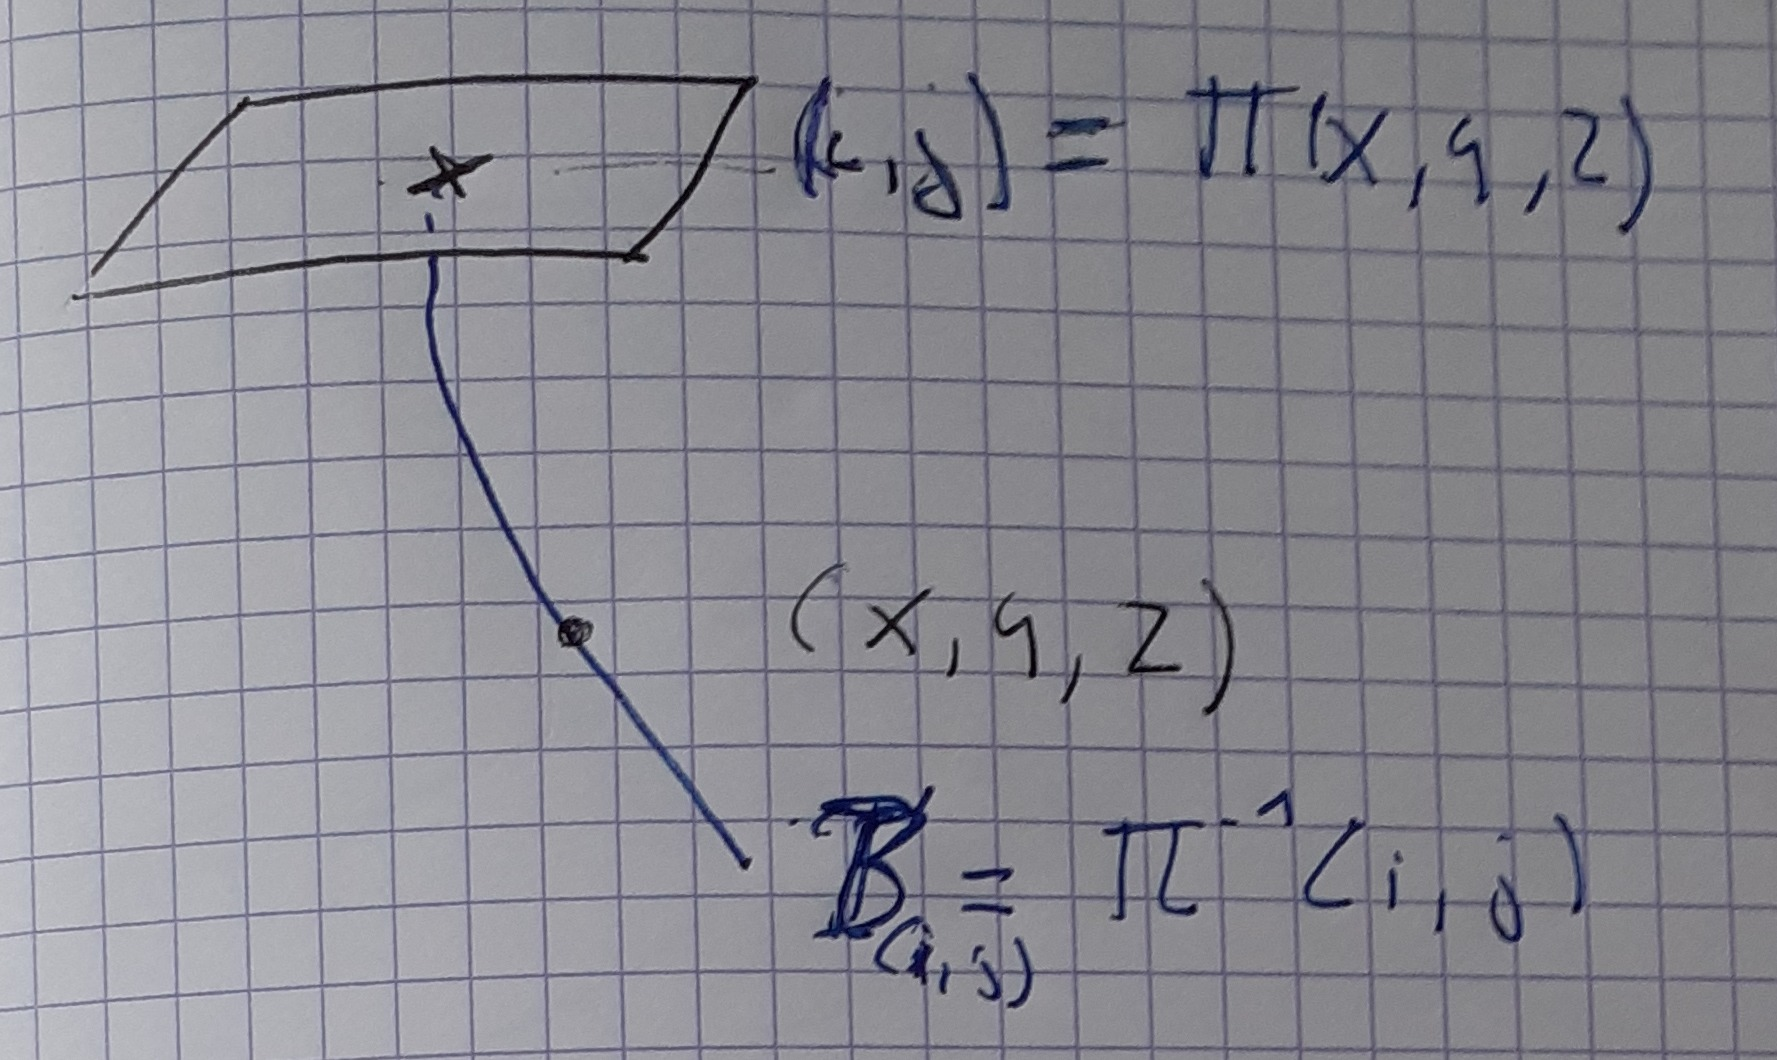
\includegraphics[width=10cm]{FIGS/NotaProj.jpg} 
 \\ \hline \hline
\end{tabular}
\caption{A projection and a bundle}
\label{FigNotaProj}
\end{figure}



%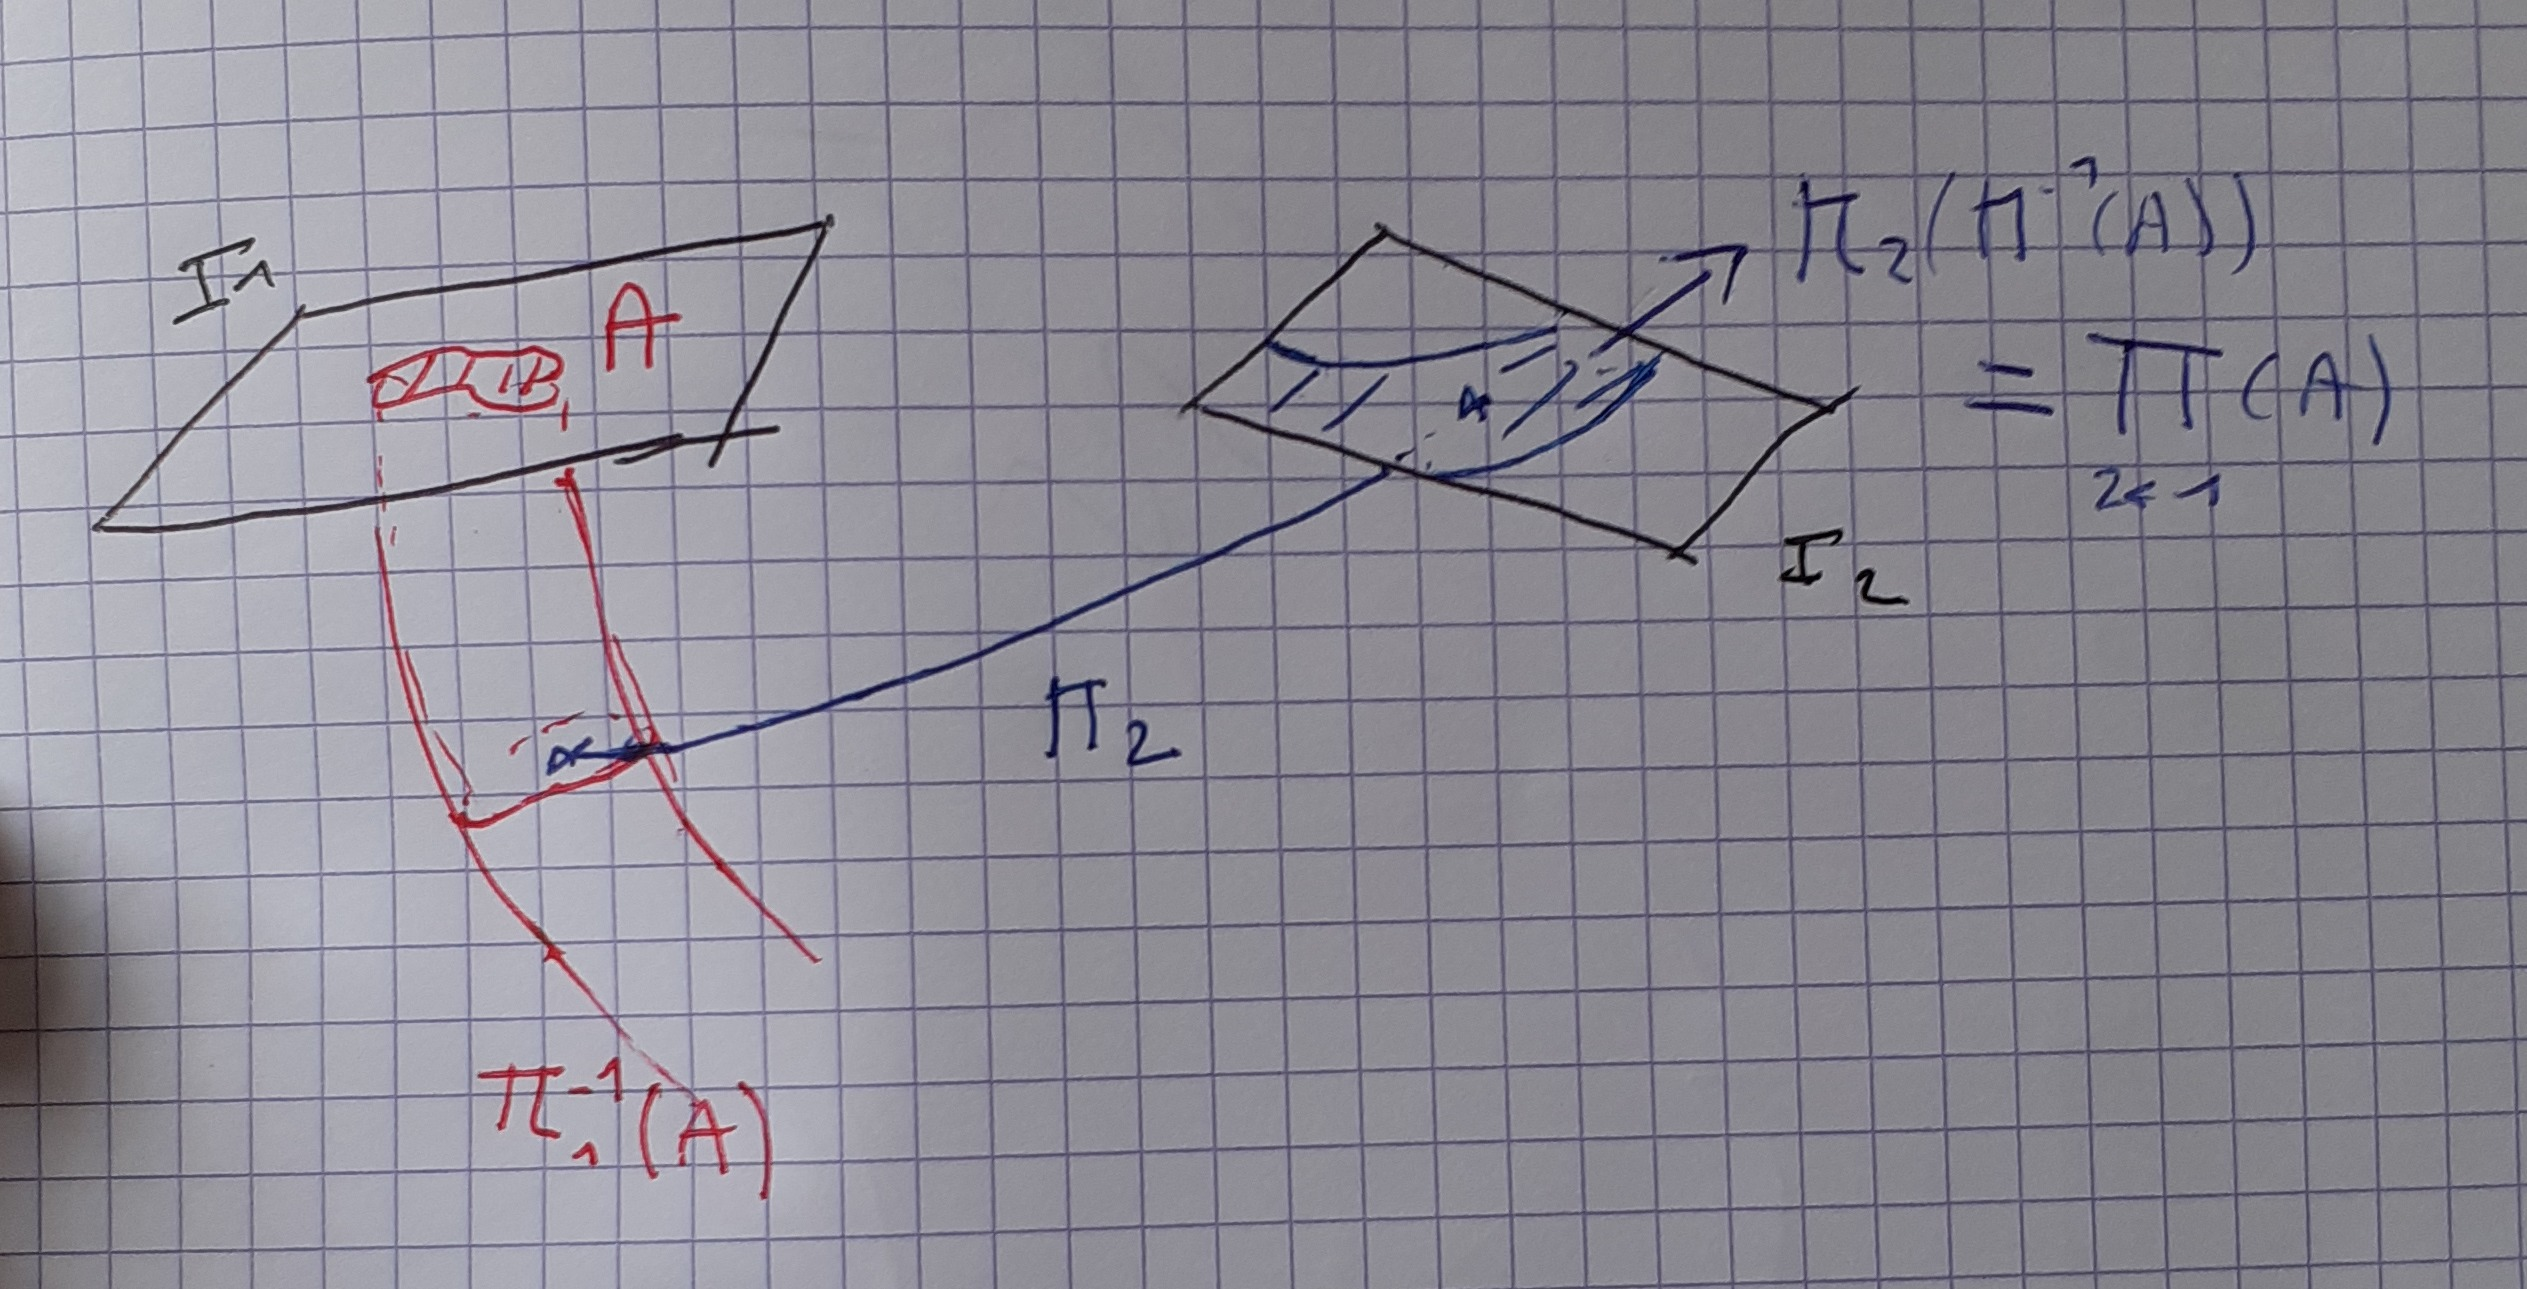
\includegraphics[width=12cm]{FIGS/NotaSets.jpg}

We define a geometric sensor of an image by a projection fonction $\pi$ that compute for a given $3d$
points its projection in image :

\begin{definition}[Generic geometric sensor model]  

\emph{Illustrated on figure\ref{FigNotaProj}}

A geometric sensor model $\pi$ is a $\mathcal{C}^{\infty}$ mapping from 
ground space ($\RR^3$) to image space (($\RR^2$) :

\begin{equation}
  \pi :  \RR^3  \rightarrow \RR^2  ,  (X,Y,Z)  \rightarrow (i,j) = \pi(X,Y,Z) \label{Eq:Proj}
\end{equation}
\end{definition}

We define the bundles of a projection :

\begin{definition}[Bundle]
For $p_k \in I_k$ we note $\BundK(p_k)$  the bundle $\pi_k^{-1}(p_k)$. When there is no confusion,
we note identically  $\BundK(P)$, with $P\in \RR^3$,
 the bundle $\pi_k^{-1}(\pi_k(P)) = \BundK(\pi_k(P))$
\end{definition}


Later, for simplicity we will use the  sub-vertical hypothesis, which allows to extend $\pi$ to a
bijective mapping of $\RR^3$ and compute its inverse  :

\begin{definition}[Subvertical camera model]  
We say that the projection is subvertical if the following mapping $\PiVert$ is a diffeomophism of $\RR^3$:
\begin{equation}
  \PiVert :  \RR^3  \rightarrow \RR^3  ,  (X,Y,Z)  \rightarrow (i,j,Z) = \PiVert(X,Y,Z)  , with (i,j) = \pi(X,Y,Z) \label{PiInvert}
\end{equation}
\end{definition}

Given $2$ images $I_1$ and $I_2$, the knowledge  of their geometric models $\pi_1$ and  $\pi_2$
reduces the matching between $2$ images to a $1d$ problem. In fact, given a point $p_1$ in $I_1$,
we can compute the $3d$ curve $\BundO(p_1)$ of  ground points that project to $p_1$ in $I_1$, and compute its
homologous curve in $I_2$ with $\pi_2(\BundO(p_1))$.



We define the H-compatible relation betwen two points
by the following definition :

\begin{definition}[H-Compatible,$\HComp$] 
\emph{Illustrated on figure\ref{FigNotaComp}}

We says that $p_1$ in  $I_1$ and $p_2$ in $I_2$ are  $\pi_1-\pi_2$ H-compatible , and write $p_1 \HComp p_2$, if   the following condition is satisified:

\begin{equation}
   ( \BundO(p_1) \cap  \BundT(p_2) \neq \emptyset    )
    \Leftrightarrow
  (\exists P \in  \RR^3 : \pi_1(P) =p_1 ,  \pi_2(P) = p_2)
\end{equation}
\end{definition}

\begin{figure}
\centering
\begin{tabular}{||c||}
 \hline \hline
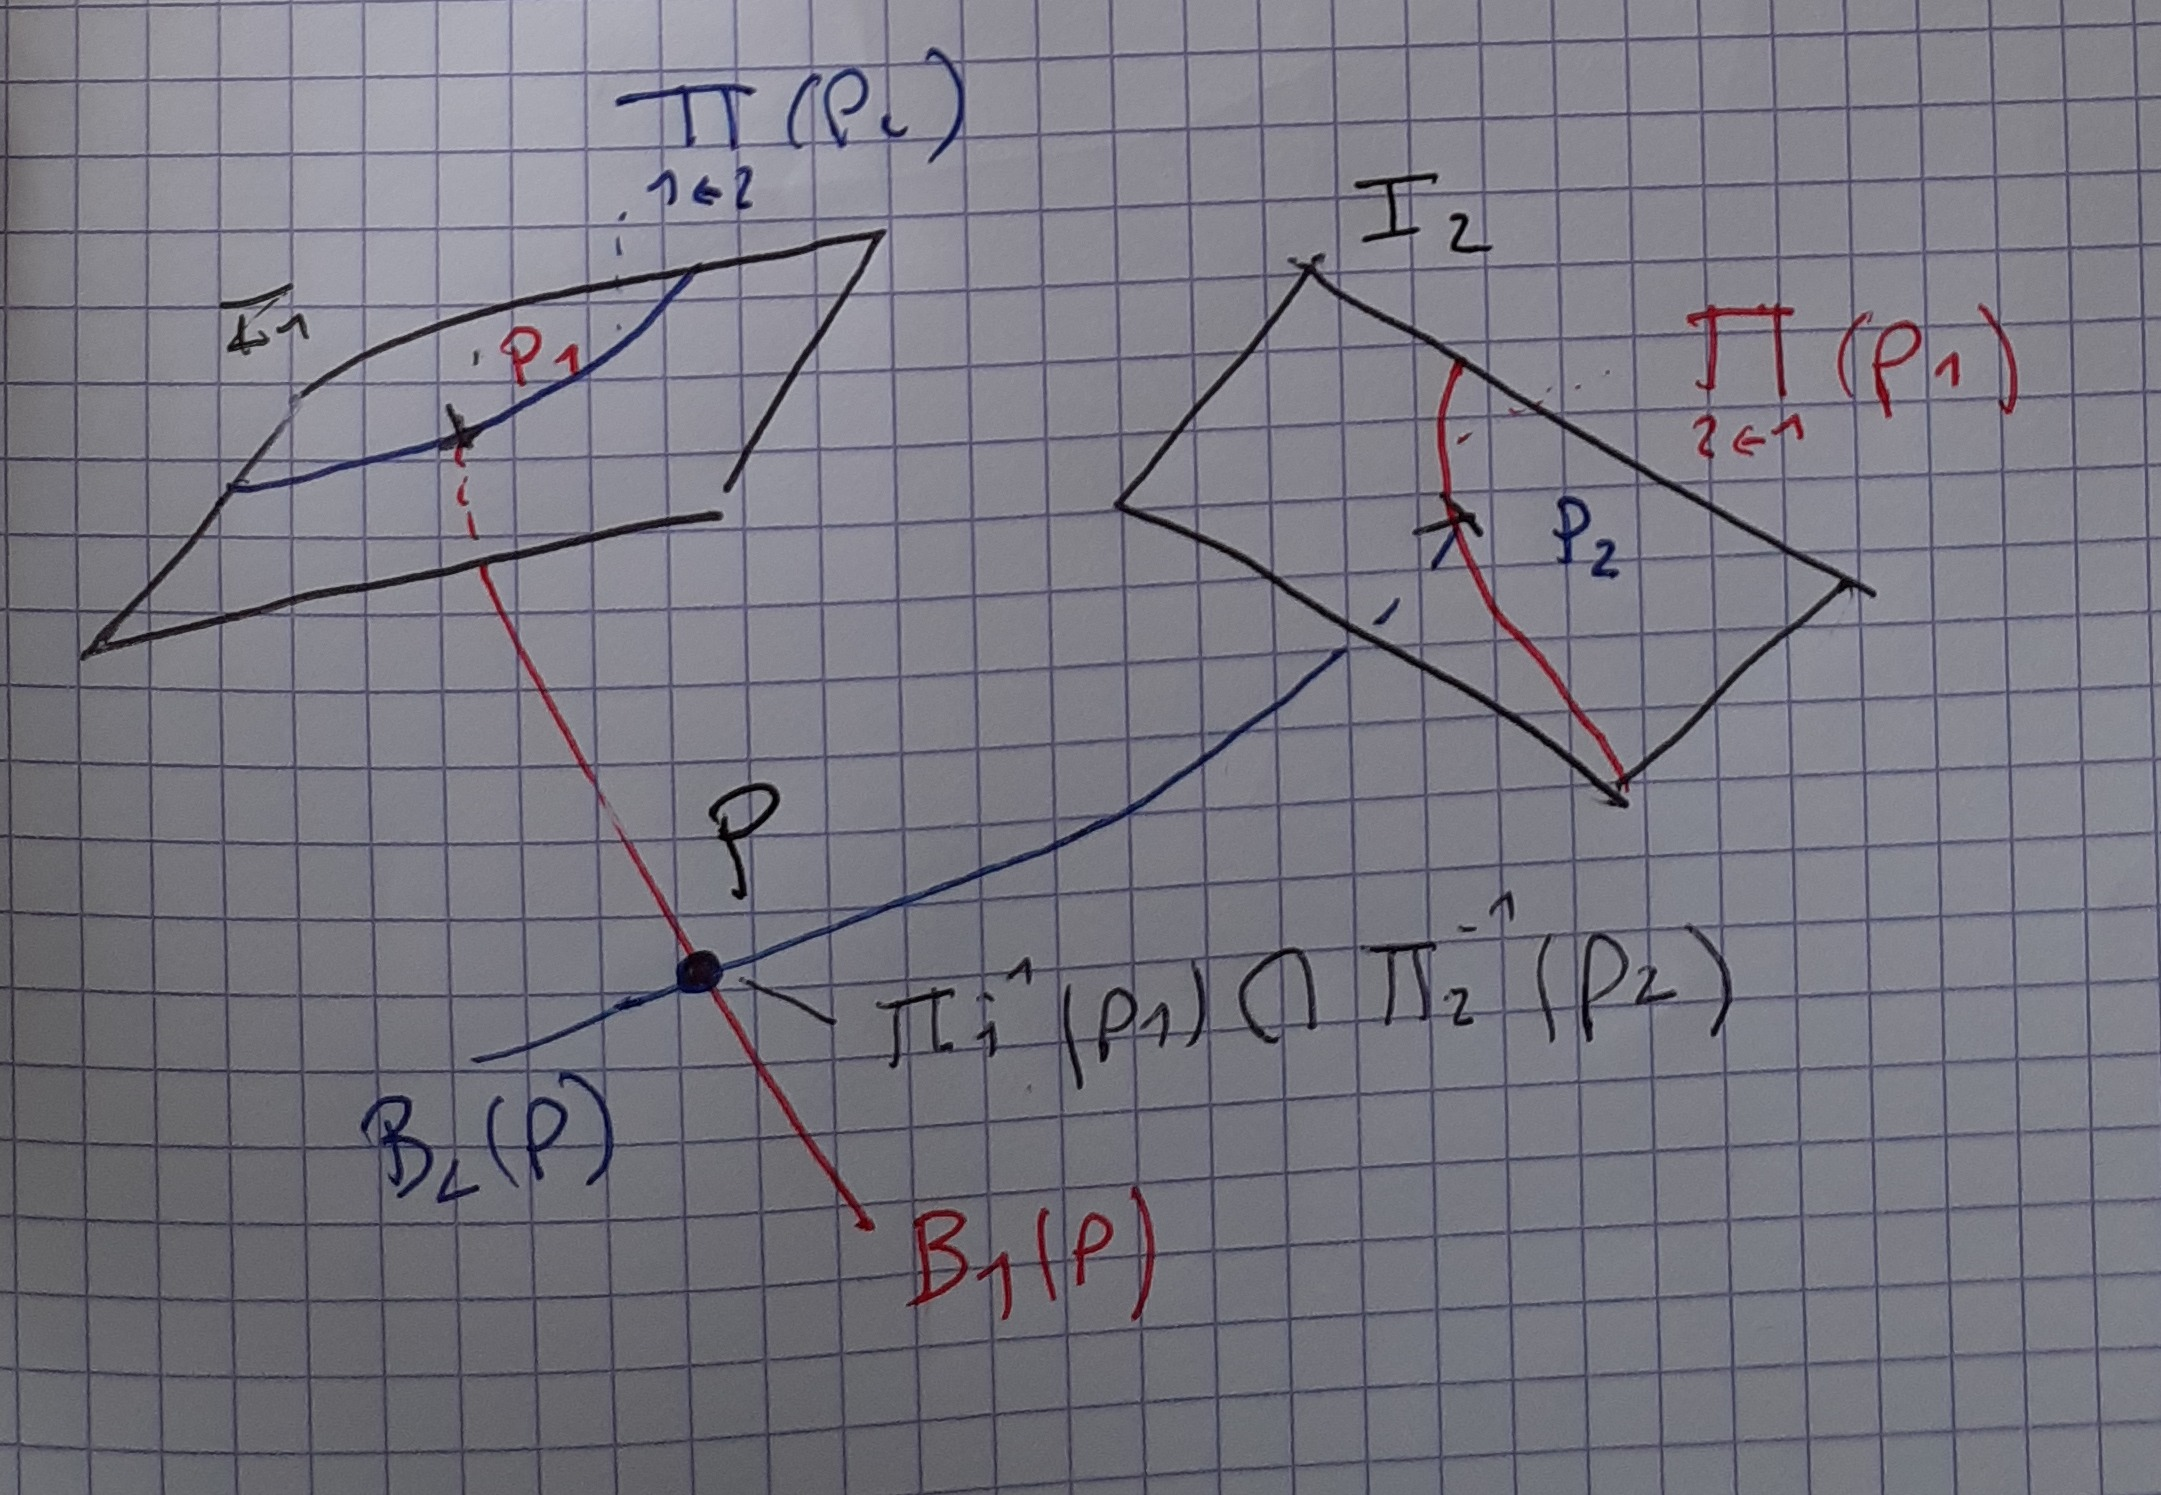
\includegraphics[width=15cm]{FIGS/NotaBundle.jpg} 
 \\ \hline \hline
\end{tabular}
\caption{Illustration of $\HComp$}
\label{FigNotaComp}
\end{figure}

In image macthing, the relation $p_1 \HComp p_2$  means that $p_1$ and $p_2$ are potentially homologous.

%---------------------------------------------
%---------------------------------------------
%---------------------------------------------



% - - - - - - - - - - - - - - -
\subsection{Definition of epipolar ressampling}

In fact, the previous relation are sufficient to implement all the matching techniques and
$(\pi_1,\pi_2)$ can be used to define a matching process taking advantage
of the~\emph{a priori} knowledge on geometry : given a point in one image, we can easily
follow its curve of  homologous compatible points in the other image.
This way of handling geometry (without epipolar) has also the advantage that it can be used in
multi image matching.  So in some way, epipolar geometry is not fundamentally required in image matching
process.

However the drawback of such approach is that it mixes in the same programm two 
different problems : the handling of geometry and ressampling on one side,
the matching process on the other side. This is here that, when one is interested
by the matching of a single pair of images, epipolar resampling
can provide an "elegant" solution for separating in two independant problems.  Traditionnaly
in epipolar geometry, two points $p_1,p_2$ are potential homologous iff they have the
same ordinate ($y_1=y_2$).

\begin{definition}[Epipolar Ressampling-1] 
\emph{Illustrated on figure~\ref{FigDefEpip} and~\ref{FigAmbigEpip}}

Let $\pi_1,\pi_2$ be two camera, let $\phi_1,\phi_2$  be two diffeomorphism
of $\RR^2$, we say that $\phi_1,\phi_2$  is an epipolar  resampling iff :

\begin{equation}
  \forall e_1=(u_1,v_1) , e_2=(u_2,v_2) : (v_1=v_2)   \Leftrightarrow  (\phi_1^{-1}(e_1) \HComp \phi_2^{-1}(e_2))
\end{equation}
   \label{EqEpiEgalY}
\end{definition}

\begin{figure}
\centering
\begin{tabular}{||c||}
 \hline \hline
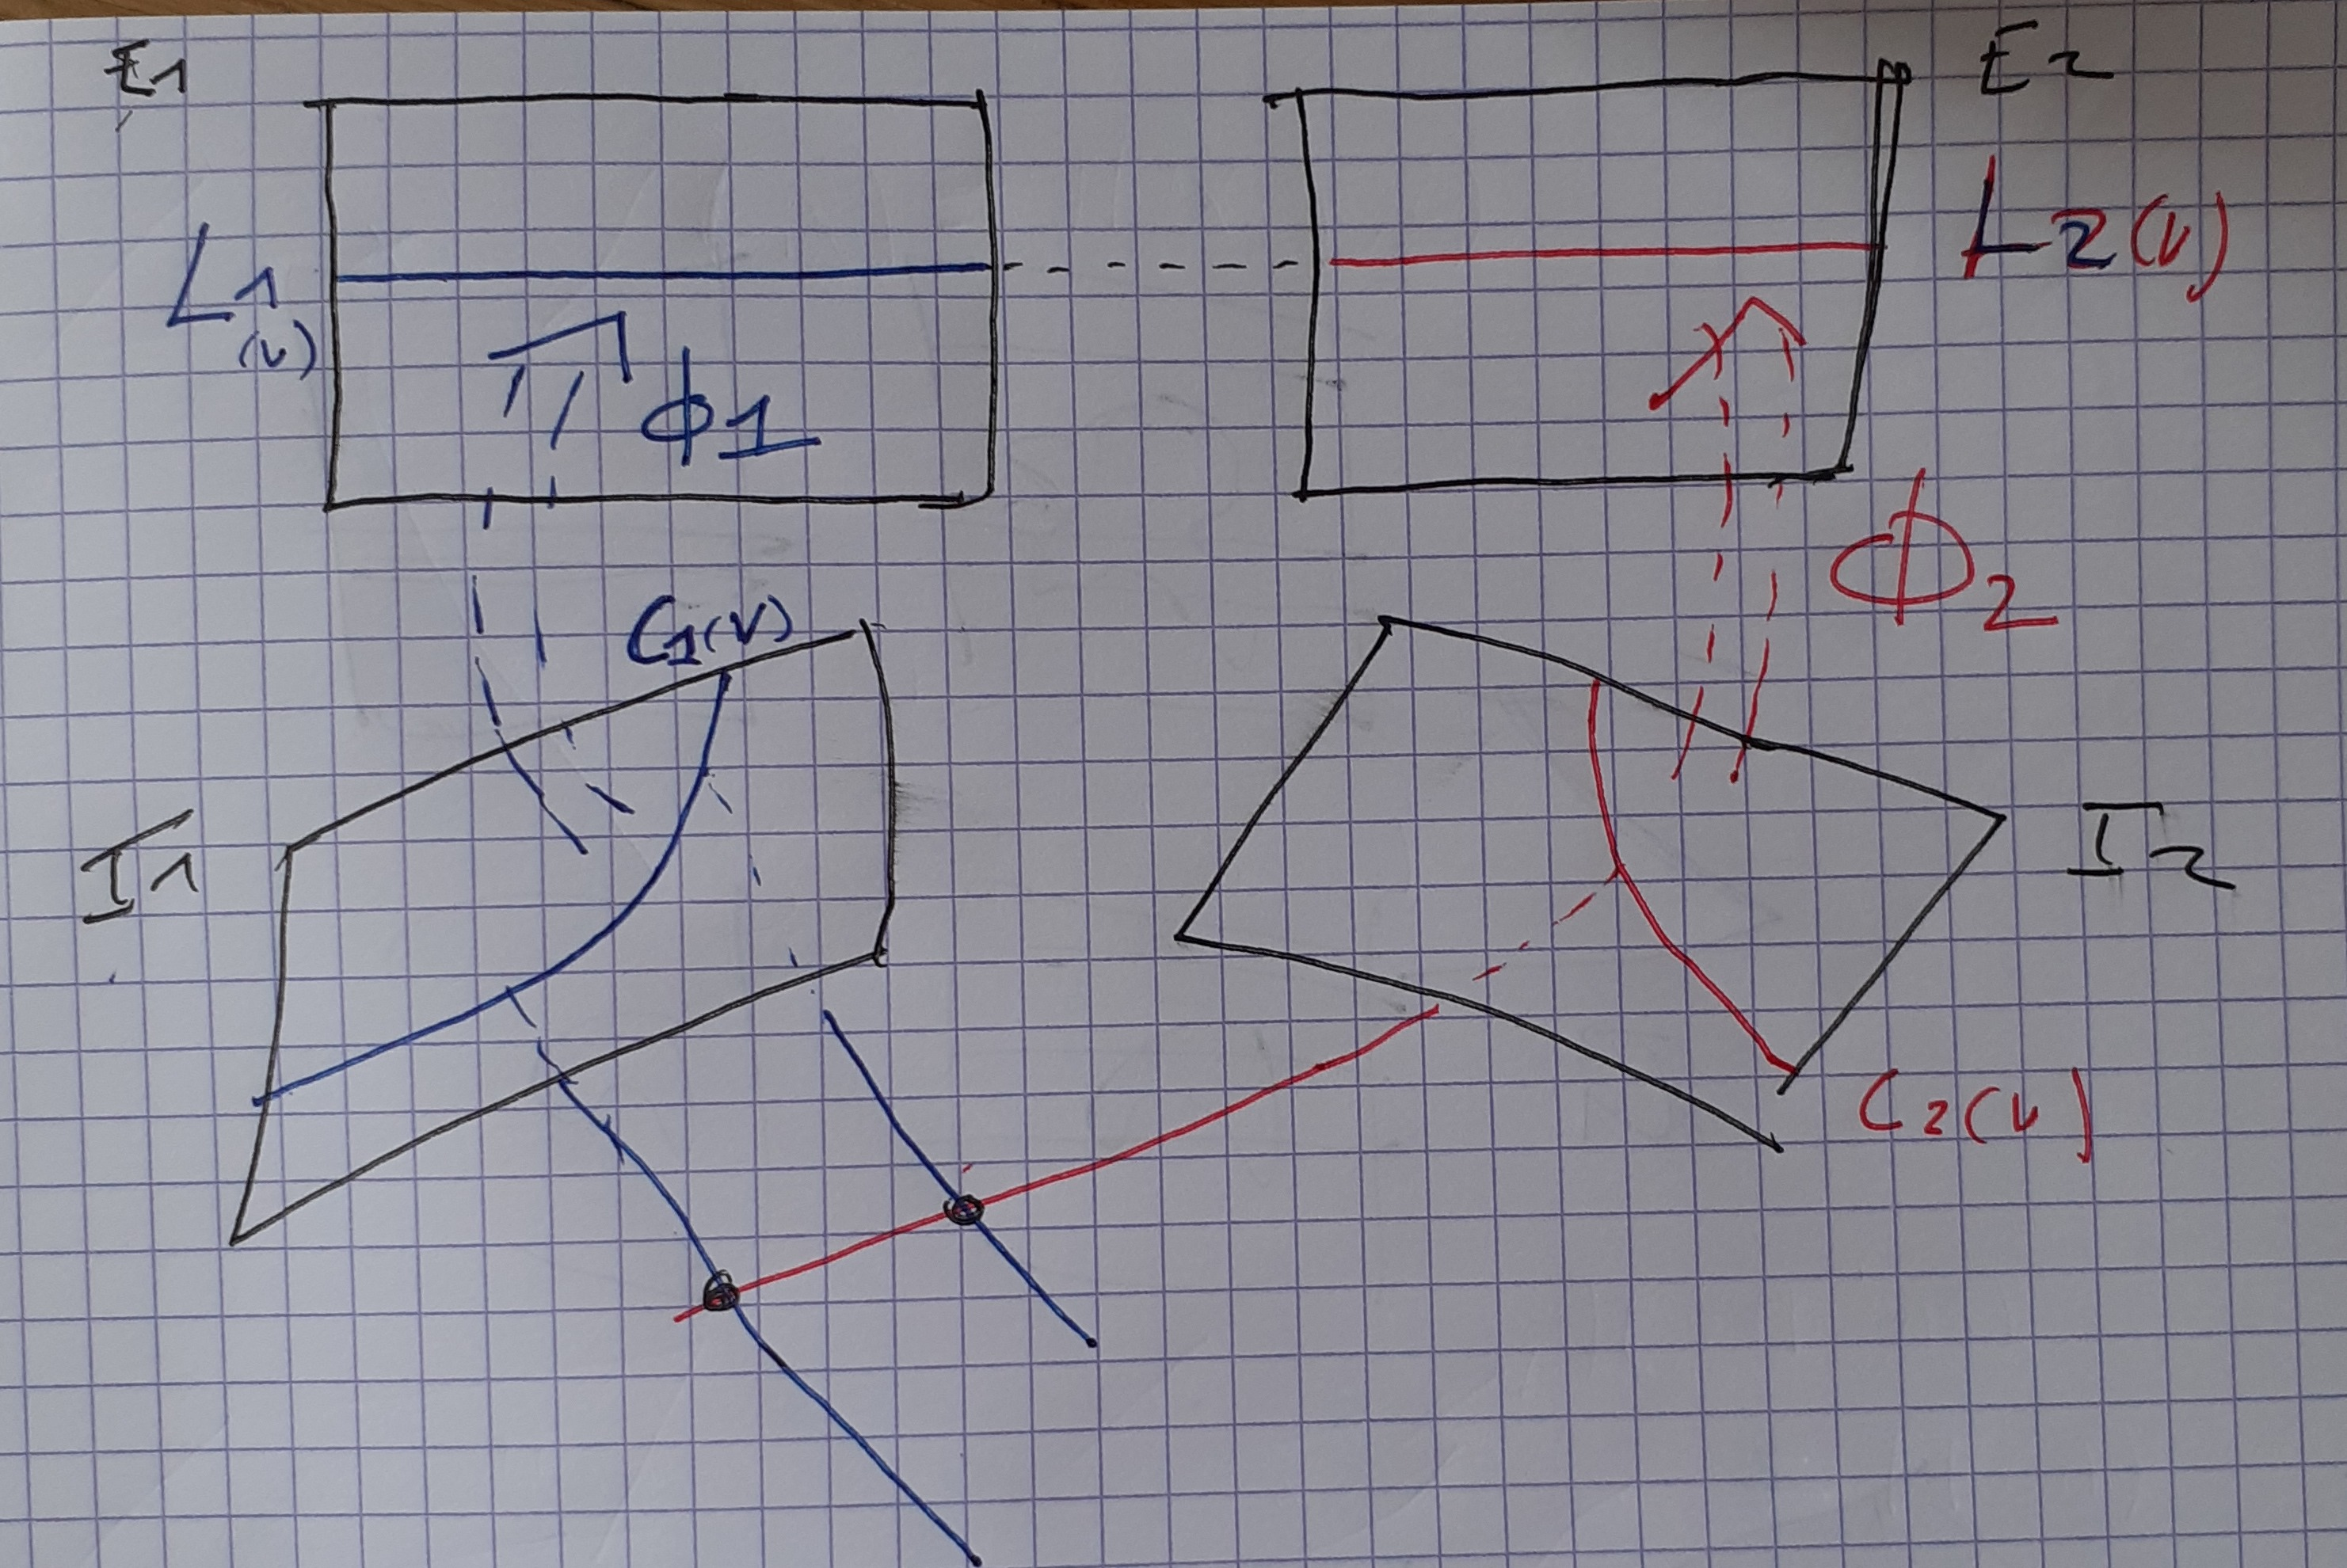
\includegraphics[width=15cm]{FIGS/Epip.jpg} 
 \\ \hline \hline
\end{tabular}
\caption{Illustration of epipolar resampling}
\label{FigDefEpip}
\end{figure}


The matching of epipolar images is facilitated as we know that globaly the lines are homologous
in two images. 

\begin{notation}[Line and curve epipolar]
We note $\LineK(v)$   the epipolar  line of $E_k$ defined by $v_k=v$. We note $\CurveK(v)$ the epipolar
curve of $I_k$ defined by $\CurveK(v) = \phi_k^{-1}(\LineK(v))$
\end{notation}


We see that when epipolar geometry exists $\CurveO(v)$ and $\CurveT(v)$ are two curves 
that are globally homologous :

\begin{equation}
     \CurveO(v) = \PiOT{C_2(v)}   ;  \CurveT(v) = \PiTO{C_1(v)} \label{Eq:CurvHom}
\end{equation}

We discuss now existence and unicity of epipolar geometry, this is important for
the theoreticall analysis of general epipolar geometry because,
as will see, epipolar geometry generally does not exist, and when it exist it is not
unique.


%---------------------------------------------

\subsection{Existence of epipolar ressampling}

\label{ExistEpip}

It is well known that :

\begin{itemize}
    \item for all pair of central projection there exist  an epipolar ressampling;

    \item  not all the pairs of geometry allow an epipolar ressampling; for example, with cylindric 
          projections, applying to many pusg-broom satellites, generally do not allow epipolar resampling;

\end{itemize}

We explain now why epipolar geometry does not exist for any $\pi_1,\pi_2$ and is rather an exception.
We define the surface $\Sv^k$ of $\RR^3$ by :

\begin{equation}
   \Sv^k = \pi_k^{-1}(\CurveK(v))  \label{Svk}
\end{equation}

Due to definition of epipolar we see that $\Sv^1$ and $\Sv^2$ are the same surface $\Sv$:

\begin{equation}
   \Sv^1 = \Sv^2 = \Sv
\end{equation}

This is a direct consequence of definitions. For any $P\in\Sv^1$, set  $e_1=\phi_1(\pi_1(P))=(u_1,v)$
and $e_2=\phi_2(\pi_2(P))=(u_2,v_2)$, whe have $\pi_1(P) \HComp \pi_2(P)$ because they are projections
of the same point, then $v_2=v$ by definition~\ref{EqEpiEgalY} and $P \in \Sv^2$.

The $\Sv$ define a foliation of $\RR^3$, and it can be seen that for any point :

\begin{equation}
   \forall v \forall P \in \Sv :  \BundO(P) \subset \Sv , \BundT \subset \Sv \label{ClothureBundle}
\end{equation}

This is again a direct consequence of definitions, if $P \in \Sv$ then $\pi_k^{-1}(P) \in \CurveK(v)$
(see equation~\ref{Svk}), then $\pi_k^{-1}(\pi_k(P)) = \BundK(P) \subset \Sv$.


But the existence of a foliation stable for the two set of bundle, as expressed in  ~\ref{ClothureBundle},
cannot  be satisfied in general, this is explained by the following arguments and illustrated 
by figure~\ref{FigClothPath}.  Let $\pi_1,\pi_2$ be two any projections and suppose
there exists  a folliation satisfying equation ~\ref{ClothureBundle} :

\begin{itemize}
   \item  let $P$ be any point of ground space, and $\Sv$ be the surface such that $P \in \Sv$;
   \item  let $P_1 \neq P$ be a point on $\BundO(P)$ , $P_1 \in \Sv$, then $\BundT(P_1) \subset \Sv$
   \item  let $P_2 \neq P$ be a point on $\BundT(P)$ , $P_2 \in S_v$, then $\BundO(P_2) \subset \Sv$
   \item  as $\BundT(P_1)$ and $\BundO(P_1)$ are included in the same surface $\Sv$ they
            must intersect somewhere in a point $Q$.
\end{itemize}

But this is the contradiction because there is no reason in general case that for any two set 
of bundles we have after this construction $\BundT(P_1) \cap \BundO(P_2) \neq \emptyset $
(see right image of figure~\ref{FigClothPath}).

\begin{figure}
\centering
\begin{tabular}{||c|c||}
 \hline \hline
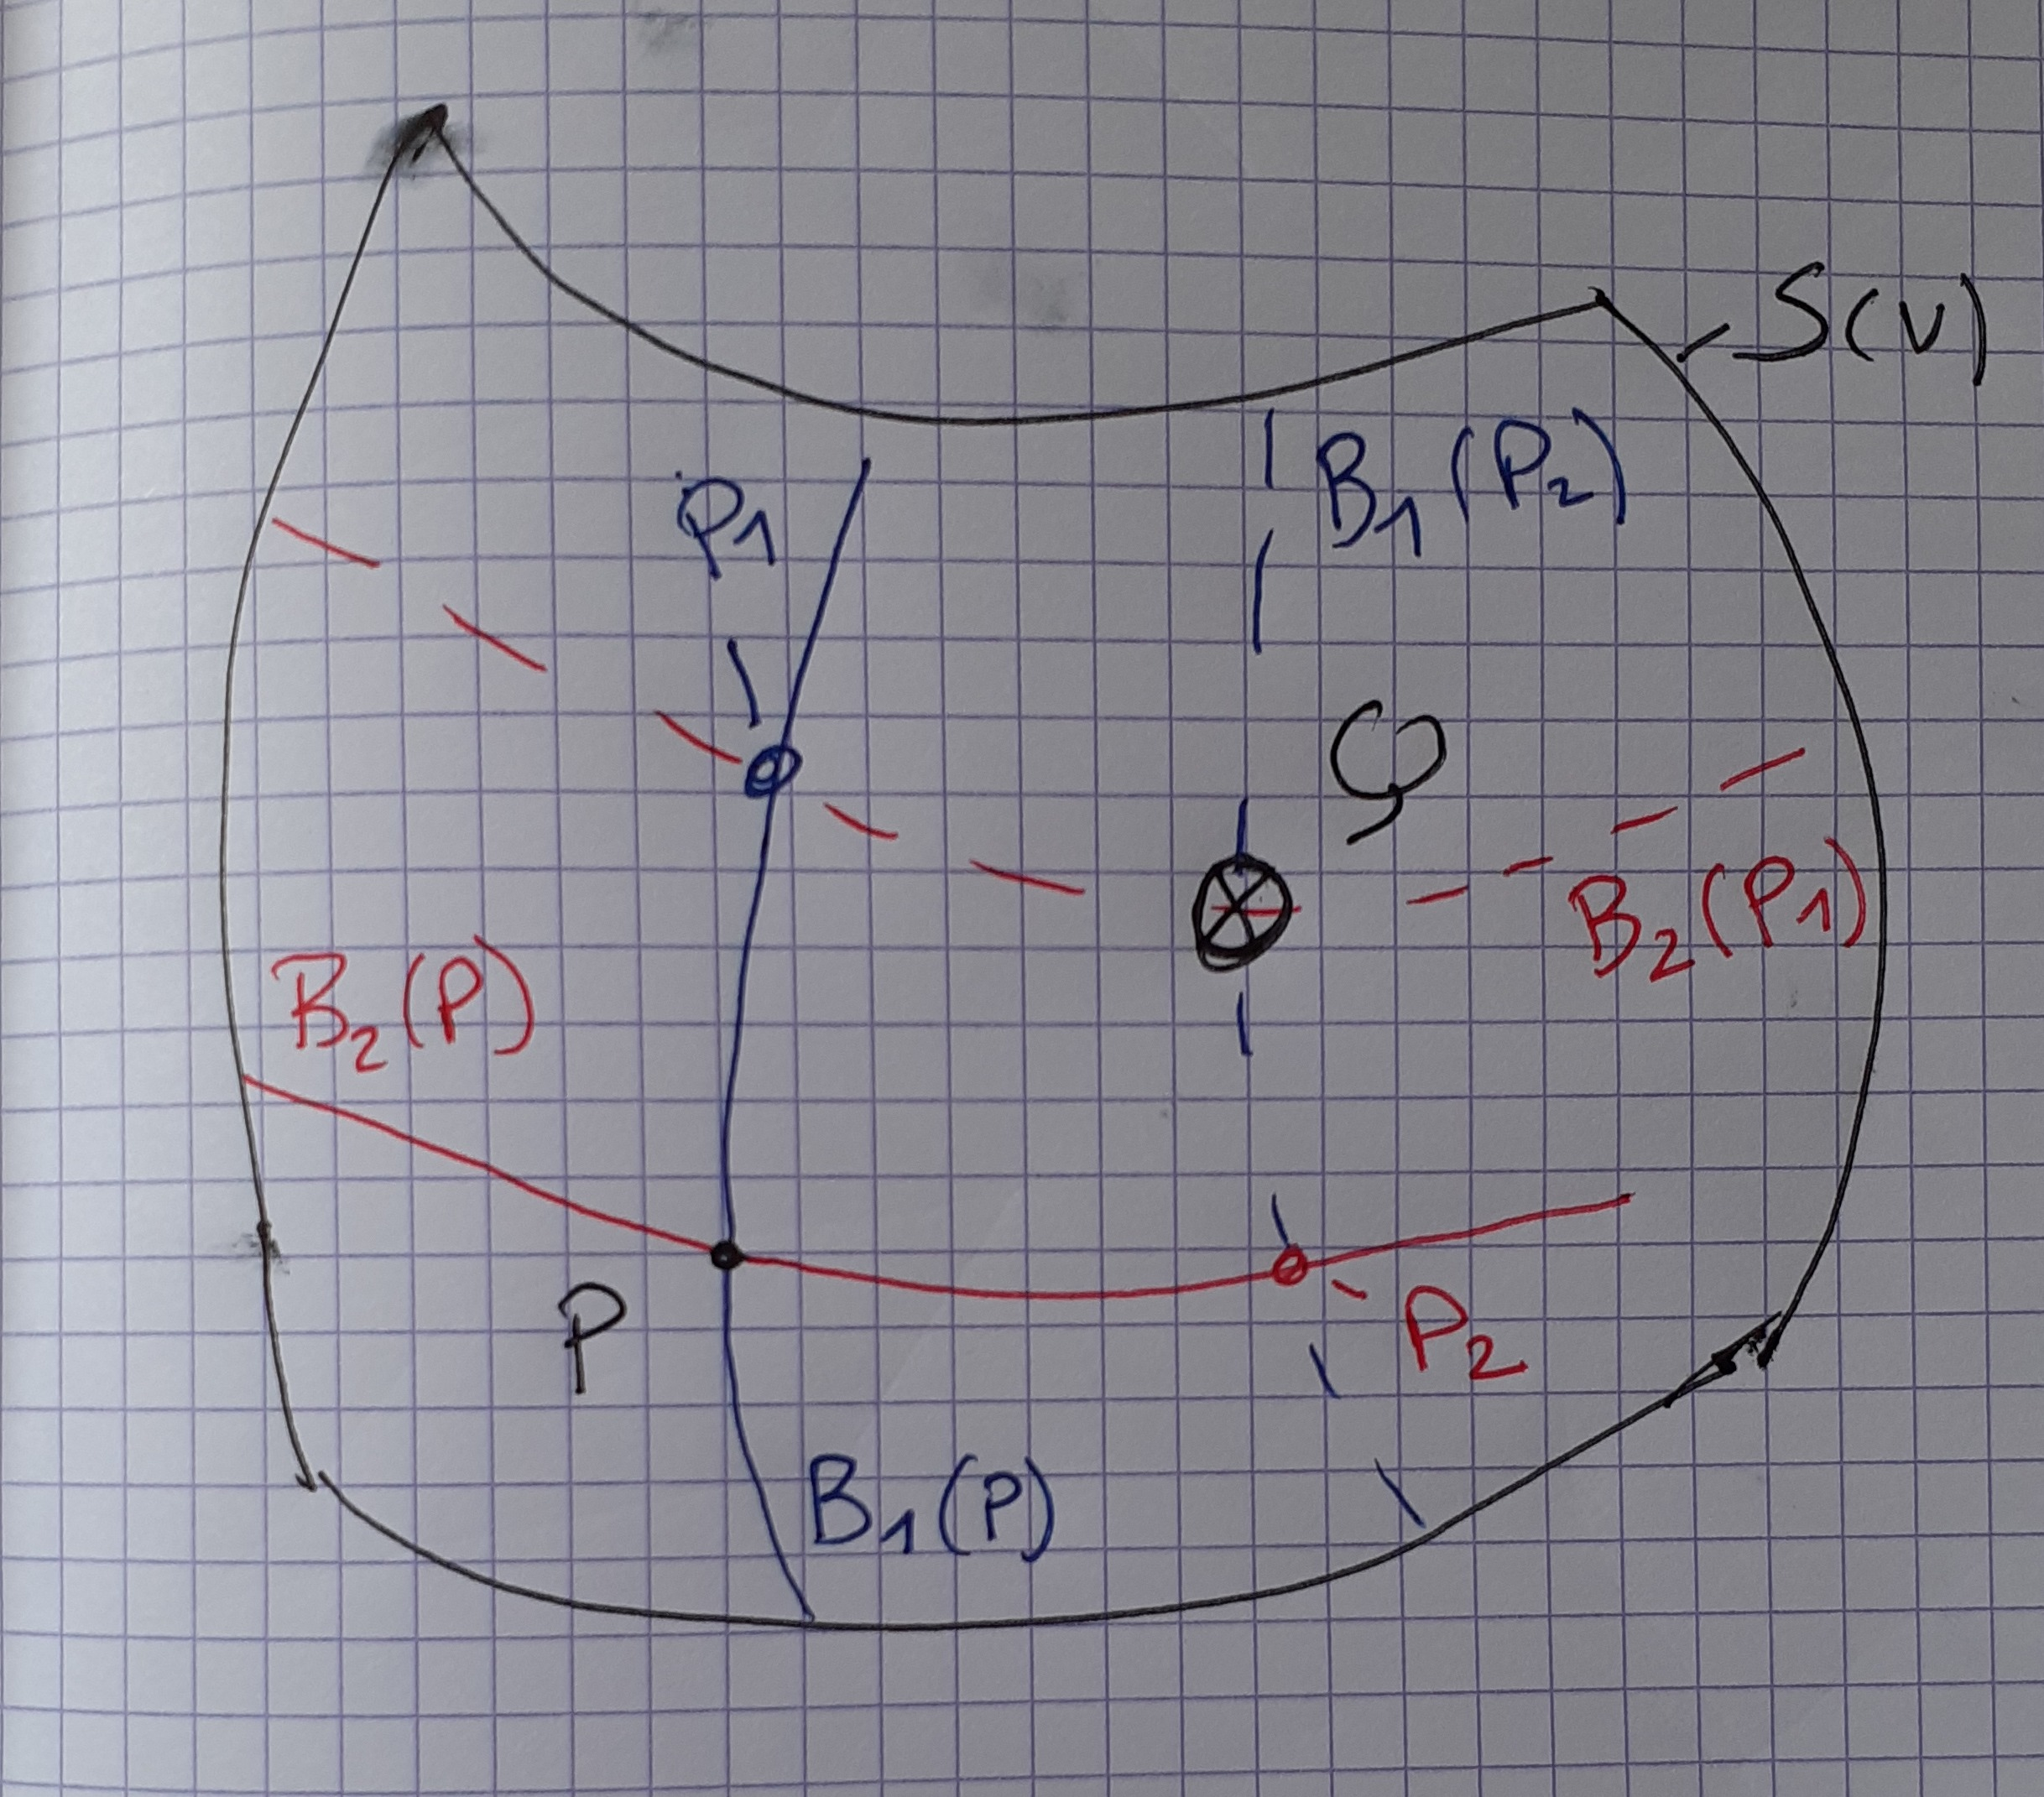
\includegraphics[width=8cm]{FIGS/ClothPathEpip.jpg} &
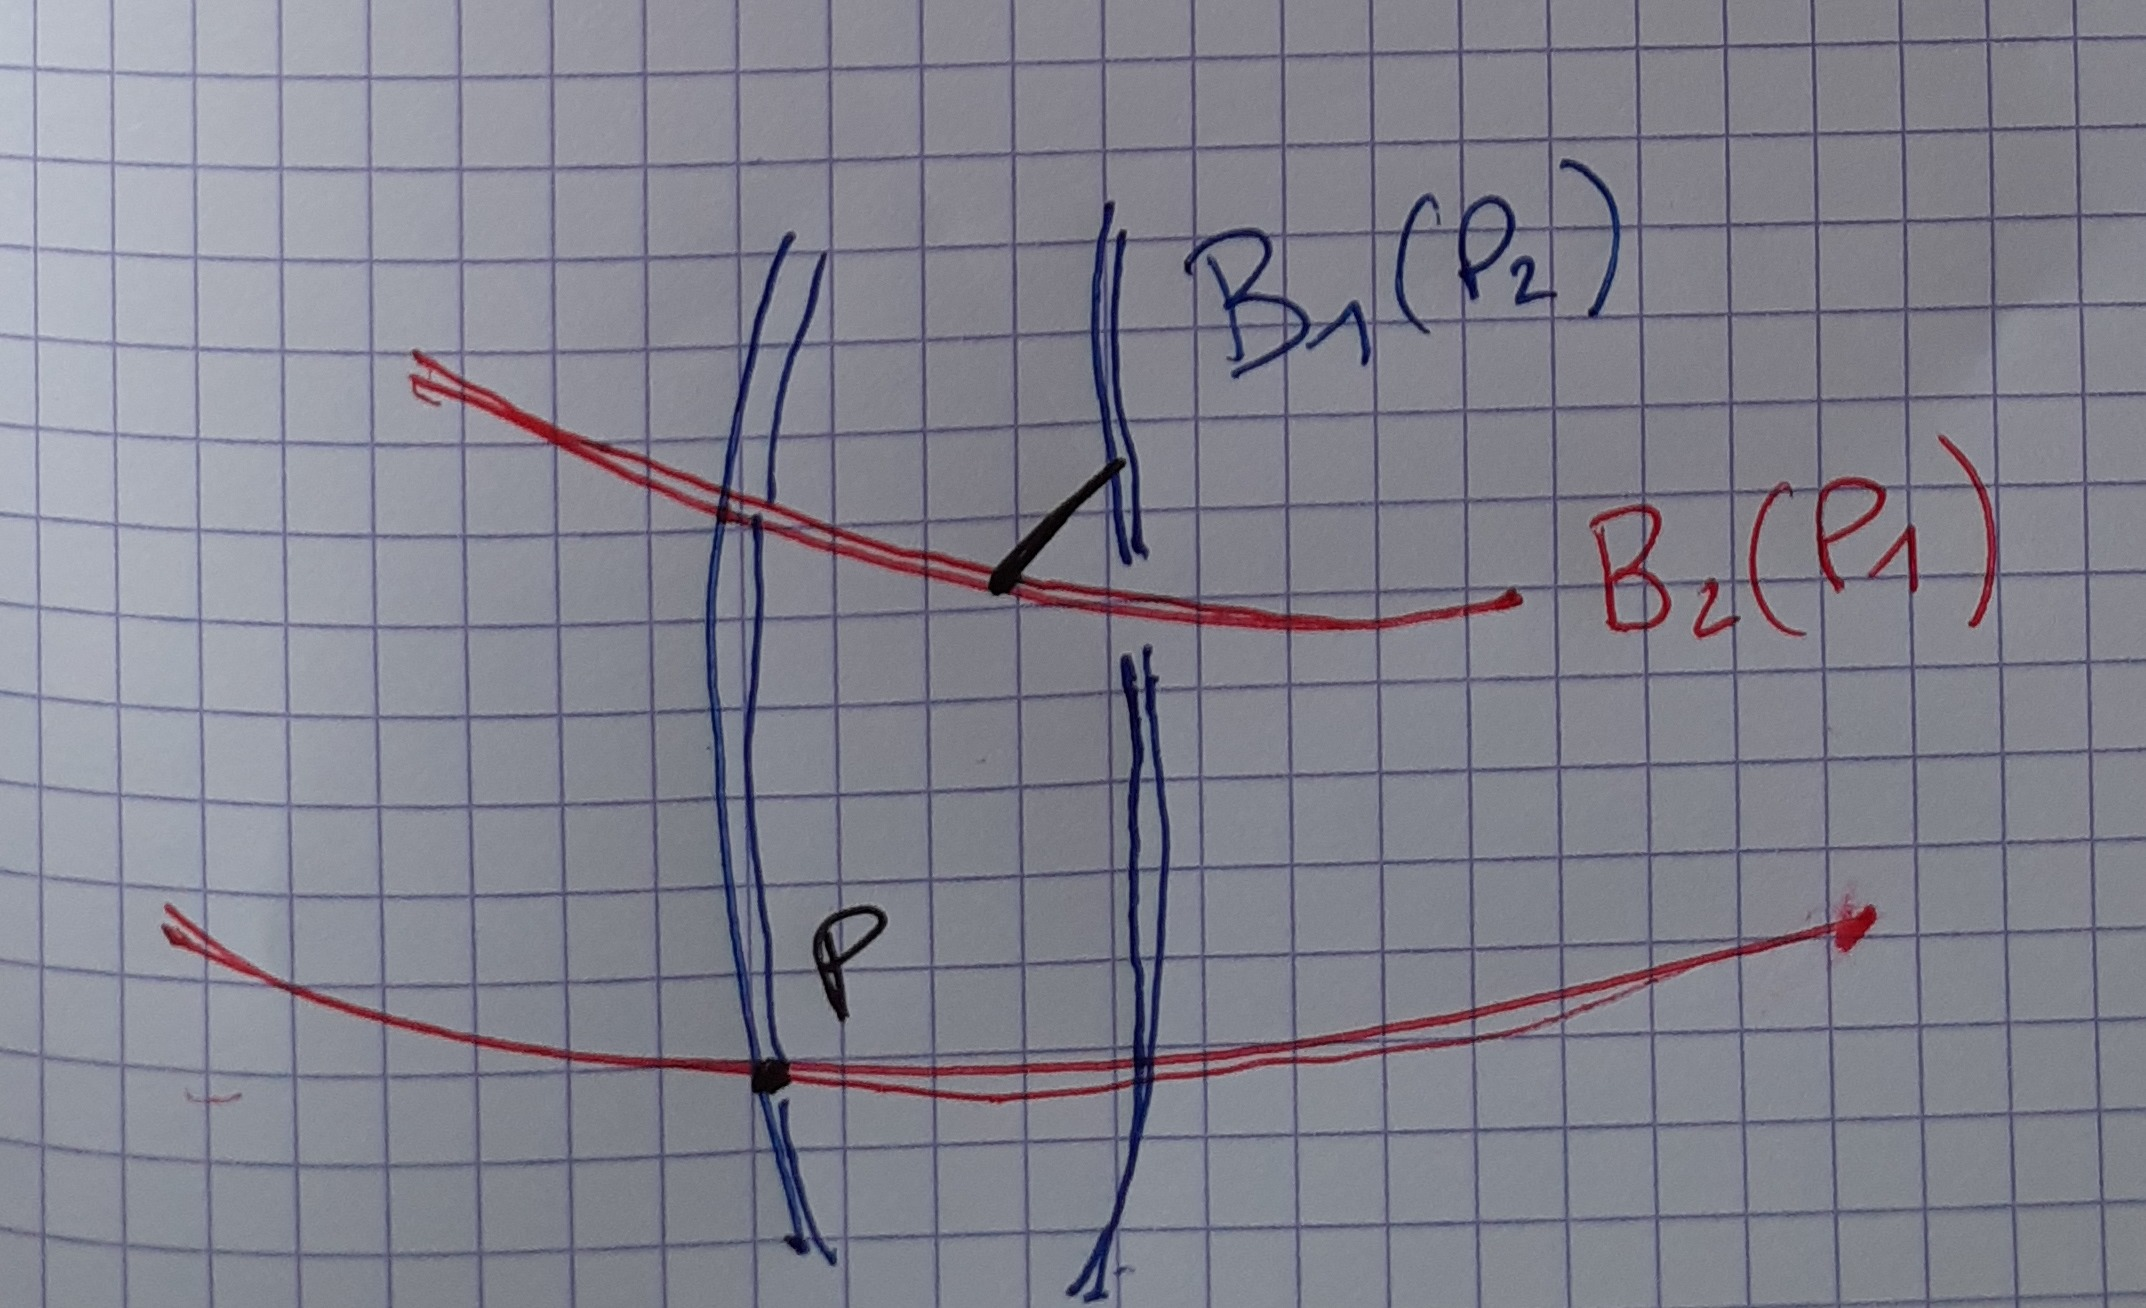
\includegraphics[width=8cm]{FIGS/ClothPathNonEpip.jpg} 
 \\ \hline \hline
\end{tabular}
\caption{Clothure of path . Left : epipolar case, the bundle are on the same level of a foliation and intersect.
Right : generic case, paht don't intersect, no epipolar can exist}
\label{FigClothPath}
\end{figure}


%---------------------------------------------


\subsection{A local caracterization of epipolar existence}

In this section we compute a local formula (i.e. a differential equation) that gives the conditions for
existence of an epipolar geometry. This section is rather theoriticall and
can be omitted for user interested mainly by practicall application.

\begin{figure}
\centering
\begin{tabular}{||c||}
 \hline \hline
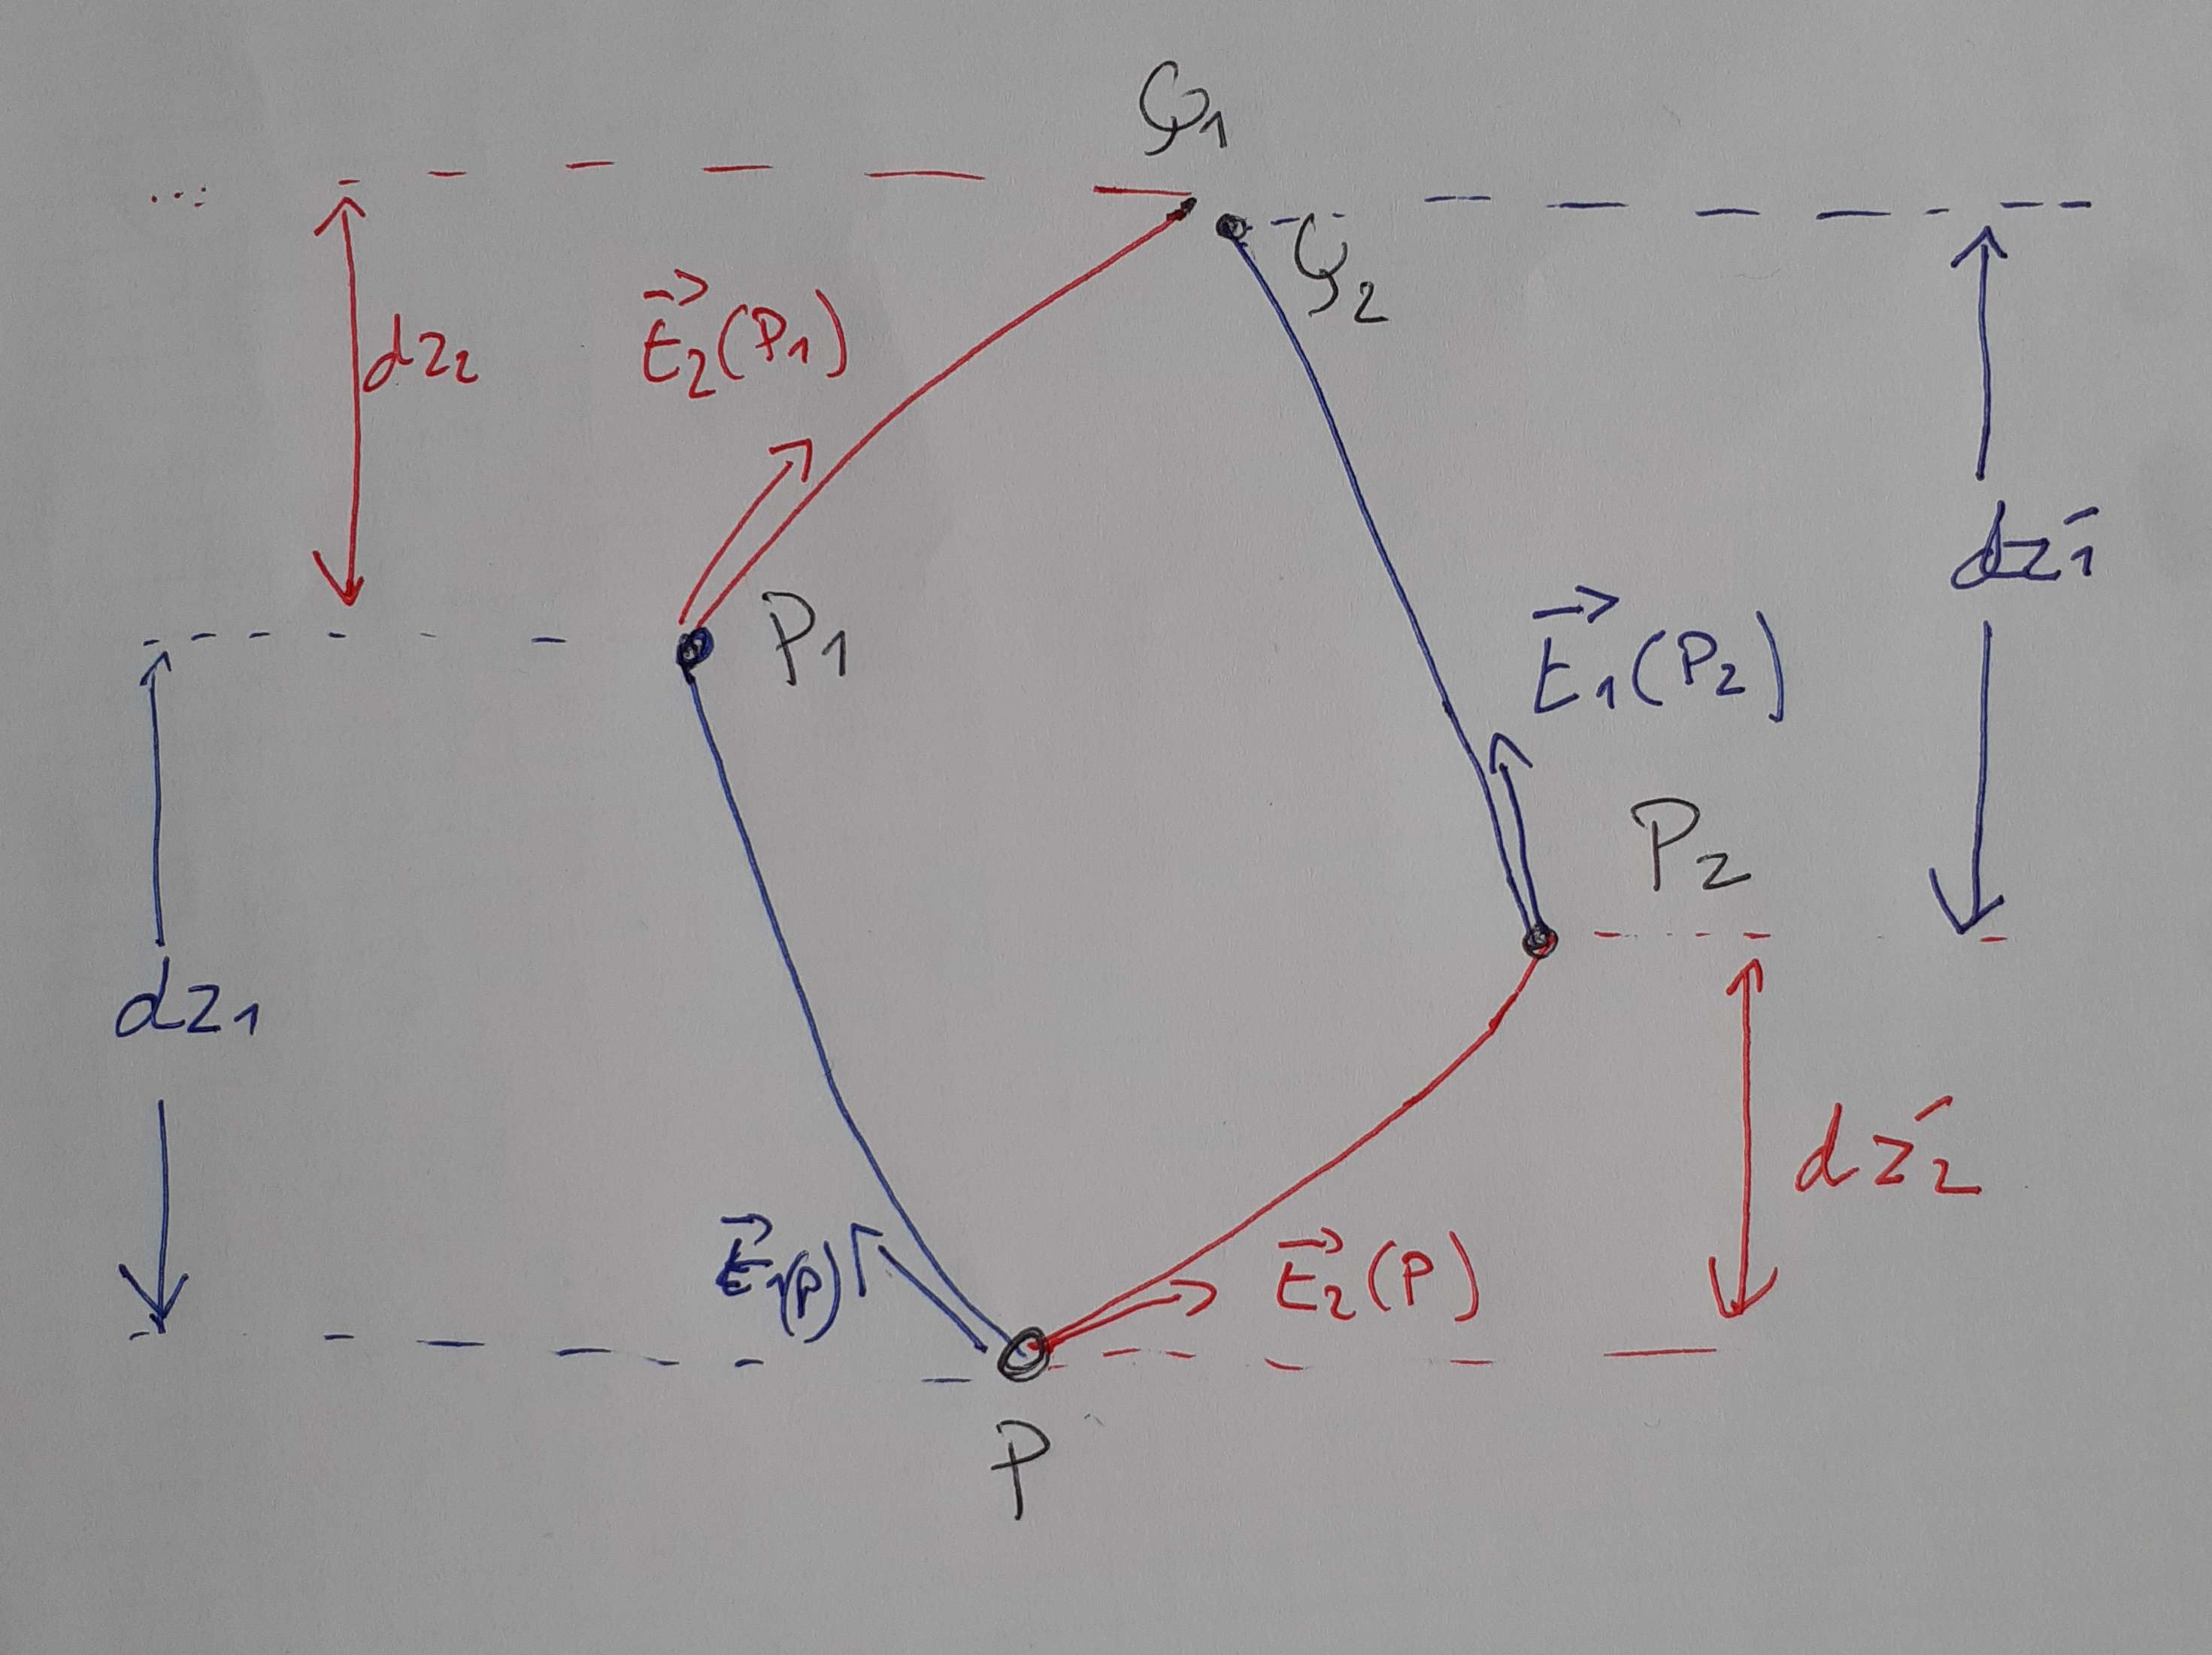
\includegraphics[width=10cm]{FIGS/EquadifEpip.jpg}
 \\ \hline \hline
\end{tabular}
\caption{Notation for local caracterization of epipolar existence}
\label{EqDifEpip}
\end{figure}

The idea is , as in section~\ref{ExistEpip}, is to make a  computation of pathes two way, $\BundO$ then $\BundT$ ,
and $\BundT$ then $\BundO$; then we express a taylor expansion of the intersection distance
between these two path.  We use the notation of figure~\ref{EqDifEpip} :

\begin{itemize}
   \item we make the sub-vertical assumption \footnote{when this assumption can be made,
          not we could use curvilinear abscisse};
   \item let $P$ be any point of $\RR^3$;
   \item consider a first path $(P,P_1,Q_1)$ following  $\BundO$ then $\BundT$ , making a
         progression $d_{z1}$ on $\BundO$ and  $d_{z2}$ on $\BundT$ ;
   \item consider a second path $(P,P_2,Q_2)$ following  $\BundT$ then $\BundO$ , making a
         progression $d_{z'2}$ on $\BundO$ and  $d_{z'1}$ on $\BundT$ ;
   \item we note $\overrightarrow{t_1(P)}=(x,y,1)$ the tangent to bundle  $\BundO$  in point $P$
         (and similarly $\overrightarrow{t_2}(P)$);
   \item when we will write  $\DerPart{F}{z_1}$ we will refer to the coordinate system $(i_1,j_1,z) = \PiVert_1^{-1}(x,y,z)$,
         idem for  $\DerPart{F}{z_2}$, and obviously as they are two different coordinate systems, we have in general
        $\DerPart{F}{z_1}  \neq \DerPart{F}{z_2}$;
\end{itemize}

Now, whatever may be the pair of 'small' values $(\delta_1,\delta_2)$,  we will compute the  pair of values
$(\delta'_1,\delta'_2)$ that minimize the distance $|Q_1,Q_2|$ and express the annulation of the
second degree taylor expansion of this distance (the first degree can always being annulated as we will see). 
Noting $\delta$ the max of all $\delta$, the degree $2$ Taylor expansion gives :

\begin{equation}
    P_1 =  P +  \delta_1 \TanO{(P)} + \frac{{\delta_1}^2}{2} \DerPart { \TanO{}}{z_1}(P)  + \Negl{\delta^3} \label{P1} 
\end{equation}
\begin{equation}
    Q_1 =  P_1 +  \delta_2 \TanT{(P_1)} + \frac{{\delta_2}^2}{2} \DerPart { \TanT{}}{z_2}(P_1) + \Negl{\delta^3} \label{Q1}
\end{equation}
\begin{equation}
     \TanT{(P_1)} = \TanT{(P)} +  \delta_1   \DerPart { \TanT{}}{z_1}(P) + \Negl{\delta^2} \label{TP1}
\end{equation}

Putting together equations~\ref{P1},~\ref{Q1},~\ref{TP1} we can make a taylor expansion of path
$P$ to $Q_1$ :

\begin{equation}
    Q_1 =    P +  \delta_1 \TanO{(P)} 
               +  \delta_2 \TanT{(P)} 
               + \frac{{\delta_1}^2}{2} \DerPart { \TanO{}}{z_1}(P) 
               + \frac{{\delta_2}^2}{2} \DerPart { \TanT{}}{z_2}(P) 
               +  \delta_1  \delta_2  \DerPart { \TanT{}}{z_1}(P)  
               + \Negl{\delta^3}
       \label{Q1ofP}
\end{equation}

And similarly for $P$ to $Q_2$ :

\begin{equation}
    Q_2 =    P +  \delta'_2 \TanT{(P)} 
               +  \delta'_1 \TanO{(P)} 
               + \frac{{\delta'_2}^2}{2} \DerPart { \TanT{}}{z_2}(P) 
               + \frac{{\delta'_1}^2}{2} \DerPart { \TanO{}}{z_1}(P) 
               +  \delta'_1  \delta'_2  \DerPart { \TanO{}}{z_2}(P)  
               + \Negl{\delta^3}
       \label{Q2ofP}
\end{equation}

The firts degree Taylor expansion of $Q_2-Q_1$ gives :

\begin{equation}
    Q_2 -Q_1 =   (\delta'_1 -\delta_1) \TanO{(P)} +  (\delta'_2 -\delta_2) \TanT{(P)}  + \Negl{\delta^2}
\end{equation}

To minimize $|Q_2 -Q_1|$, the first step is to annulate the degree $1$ terms of $ Q_2 -Q_1$ . We assume
that $\TanT{(P)}$ and $\TanO{(P)}$  are independant vectors~\footnote{elsewhere, it would be a 
degenerate case of stereovision} and we must then make of $\delta'_2 -\delta_2$ and $\delta'_1 -\delta_1$
term of degre $2$ :

\begin{equation}
   \Delta_1 =   \delta'_1 -\delta_1 = \Negl{\delta^2}  \; ; \; \Delta_2 =   \delta'_2 -\delta_2 = \Negl{\delta^2}
   \label{Delta}
\end{equation}

To develop $ Q_2 -Q_1$ we can use the following identities  that are direct consquences of~\ref{Delta} :

\begin{equation}
   \delta_1  \delta_2 -  \delta'_1  \delta'_2  = \Negl{\delta^3} \;;\;
   {\delta_1}^2 - {\delta'_1}^2 =  \Negl{\delta^3} \;;\;
   {\delta_2}^2 - {\delta'_2}^2 =  \Negl{\delta^3} 
   \label{NeglDelta}
\end{equation}

Subtracting \ref{Q1ofP} to \ref{Q2ofP}, and using~\ref{NeglDelta},we can write :

\begin{equation}
    Q_2 -Q_1 =   \Delta_1 \TanO{(P)} +   \Delta_2 \TanT{(P)}  
               + \delta_1  \delta_2(\DerPart { \TanT{}}{z_1}(P)  -\DerPart { \TanO{}}{z_2}(P) )
               + \Negl{\delta^3}
\end{equation}


We now traduce the intersection of path by annulating the degree $2$ Taylor expansion of $Q_2 -Q_1$.
We have  $3$ vector, and their weighted sum can be null, iff they are colinear.

\begin{theorem}[Existence of epipolar]
The epipolar exist iff the following determinant is null :

\begin{equation}
\left[ \begin{array}{c|c|c}
\TanO{} & \TanT{}  & \DerPart { \TanT{}}{z_1}  -\DerPart { \TanO{}}{z_2}  
\end{array} \right]  
=0
\end{equation}

\end{theorem}

\begin{remark}[Epipolar equation with central perspective camera]
As an illustration in an easy case, we can see that this condition is trivially 
satisfied for a pair of central perspective cameras as we have the annulation of both terms as shown
in equation~\ref{EqEpipConik}. This is because for a given point $P$,
for any point $P_1$ on $\BundO(P)$, $\TanT{P_1}$ belongs to the epipolar
plane $\mathcal{P}$ , we have $\TanT{P_1} \in \mathcal{P}$, so $\DerPart { \TanT{}}{z_1} \in \mathcal{P}$,
and as we have also $\TanO{(P)} \in  \mathcal{P}, \TanT{(P)} \in  \mathcal{P}$, the collineratity
between $\TanO{(P)}$ , $\TanT{(P)}$ and $\DerPart { \TanT{}}{z_1}(P)$ is proved.

\begin{equation}
\left[ \begin{array}{c|c|c}
\TanO{} & \TanT{}  & \DerPart { \TanT{}}{z_1}  
\end{array} \right]  
=\left[ \begin{array}{c|c|c}
\TanO{} & \TanT{}  & \DerPart { \TanO{}}{z_2}  
\end{array} \right]  
=0
\label{EqEpipConik}
\end{equation}
\end{remark}



%---------------------------------------------


\subsection{Ambiguity of epipolar ressampling}

When it exists, the epipolar ressembling is not unique.  We
describe here exactly the ambiguity that exists as it is necessary
to handle it rigourously in the method we propose for optimal epipolar rectification.

Let $\phi_1,\phi_2$ and  $\phi'_1,\phi'_2$ be two   epipolar resampling.
For any pair of lines $\LineK(v)$ of $E_k$, 
$\CurveO(v),\CurveT(v)$  are homologous curves of 
$I_1,I_2$ as in equation~\ref{Eq:CurvHom} .  Then $\phi'_k(\CurveK(v)))$
are   lines $\LineK(v')$ of $E_k$.
We see that $\phi'_1 \phi_1^{-1}$  and $\phi'_2 \phi_2^{-1}$ are diffeomorphism
that transform lines in lines, and that globally operate the same transformation
on lines (see figure~\ref{FigAmbigEpip}).

Conversely let   $\phi_1,\phi_2$ be an epipolar resampling, let $\Lambda_1,\Lambda_2$ 
be two diffeomorphism , stable for lines, and making globally the same transfomation on lines, we see that 
we see that $\Lambda_1 \circ \phi_1$ and  $\Lambda_2 \circ \phi_2$ are also an epipolar resampling.


Having computed exactly the ambiguity that exist on epipolar, we can now fix the constraints to impose 
for having an unique epipolar resampling : (1) regarding the unicity  of the deformation
inside each line of each function, we can impose the constraint that the colums stay stable (i.e.
the deformation is made only on  $y$), this the contraint of equations~\ref{Ambig:PhiO}
and~\ref{Ambig:PhiT}, (2) regarding the global deformation of lines \footnote{i.e. where each line
is transformed globally to another line} we must fix the transformation  for one image,
this done by equation~\ref{FigAmbigEpip}.

\begin{figure}
\centering
\begin{tabular}{||c||}
 \hline \hline
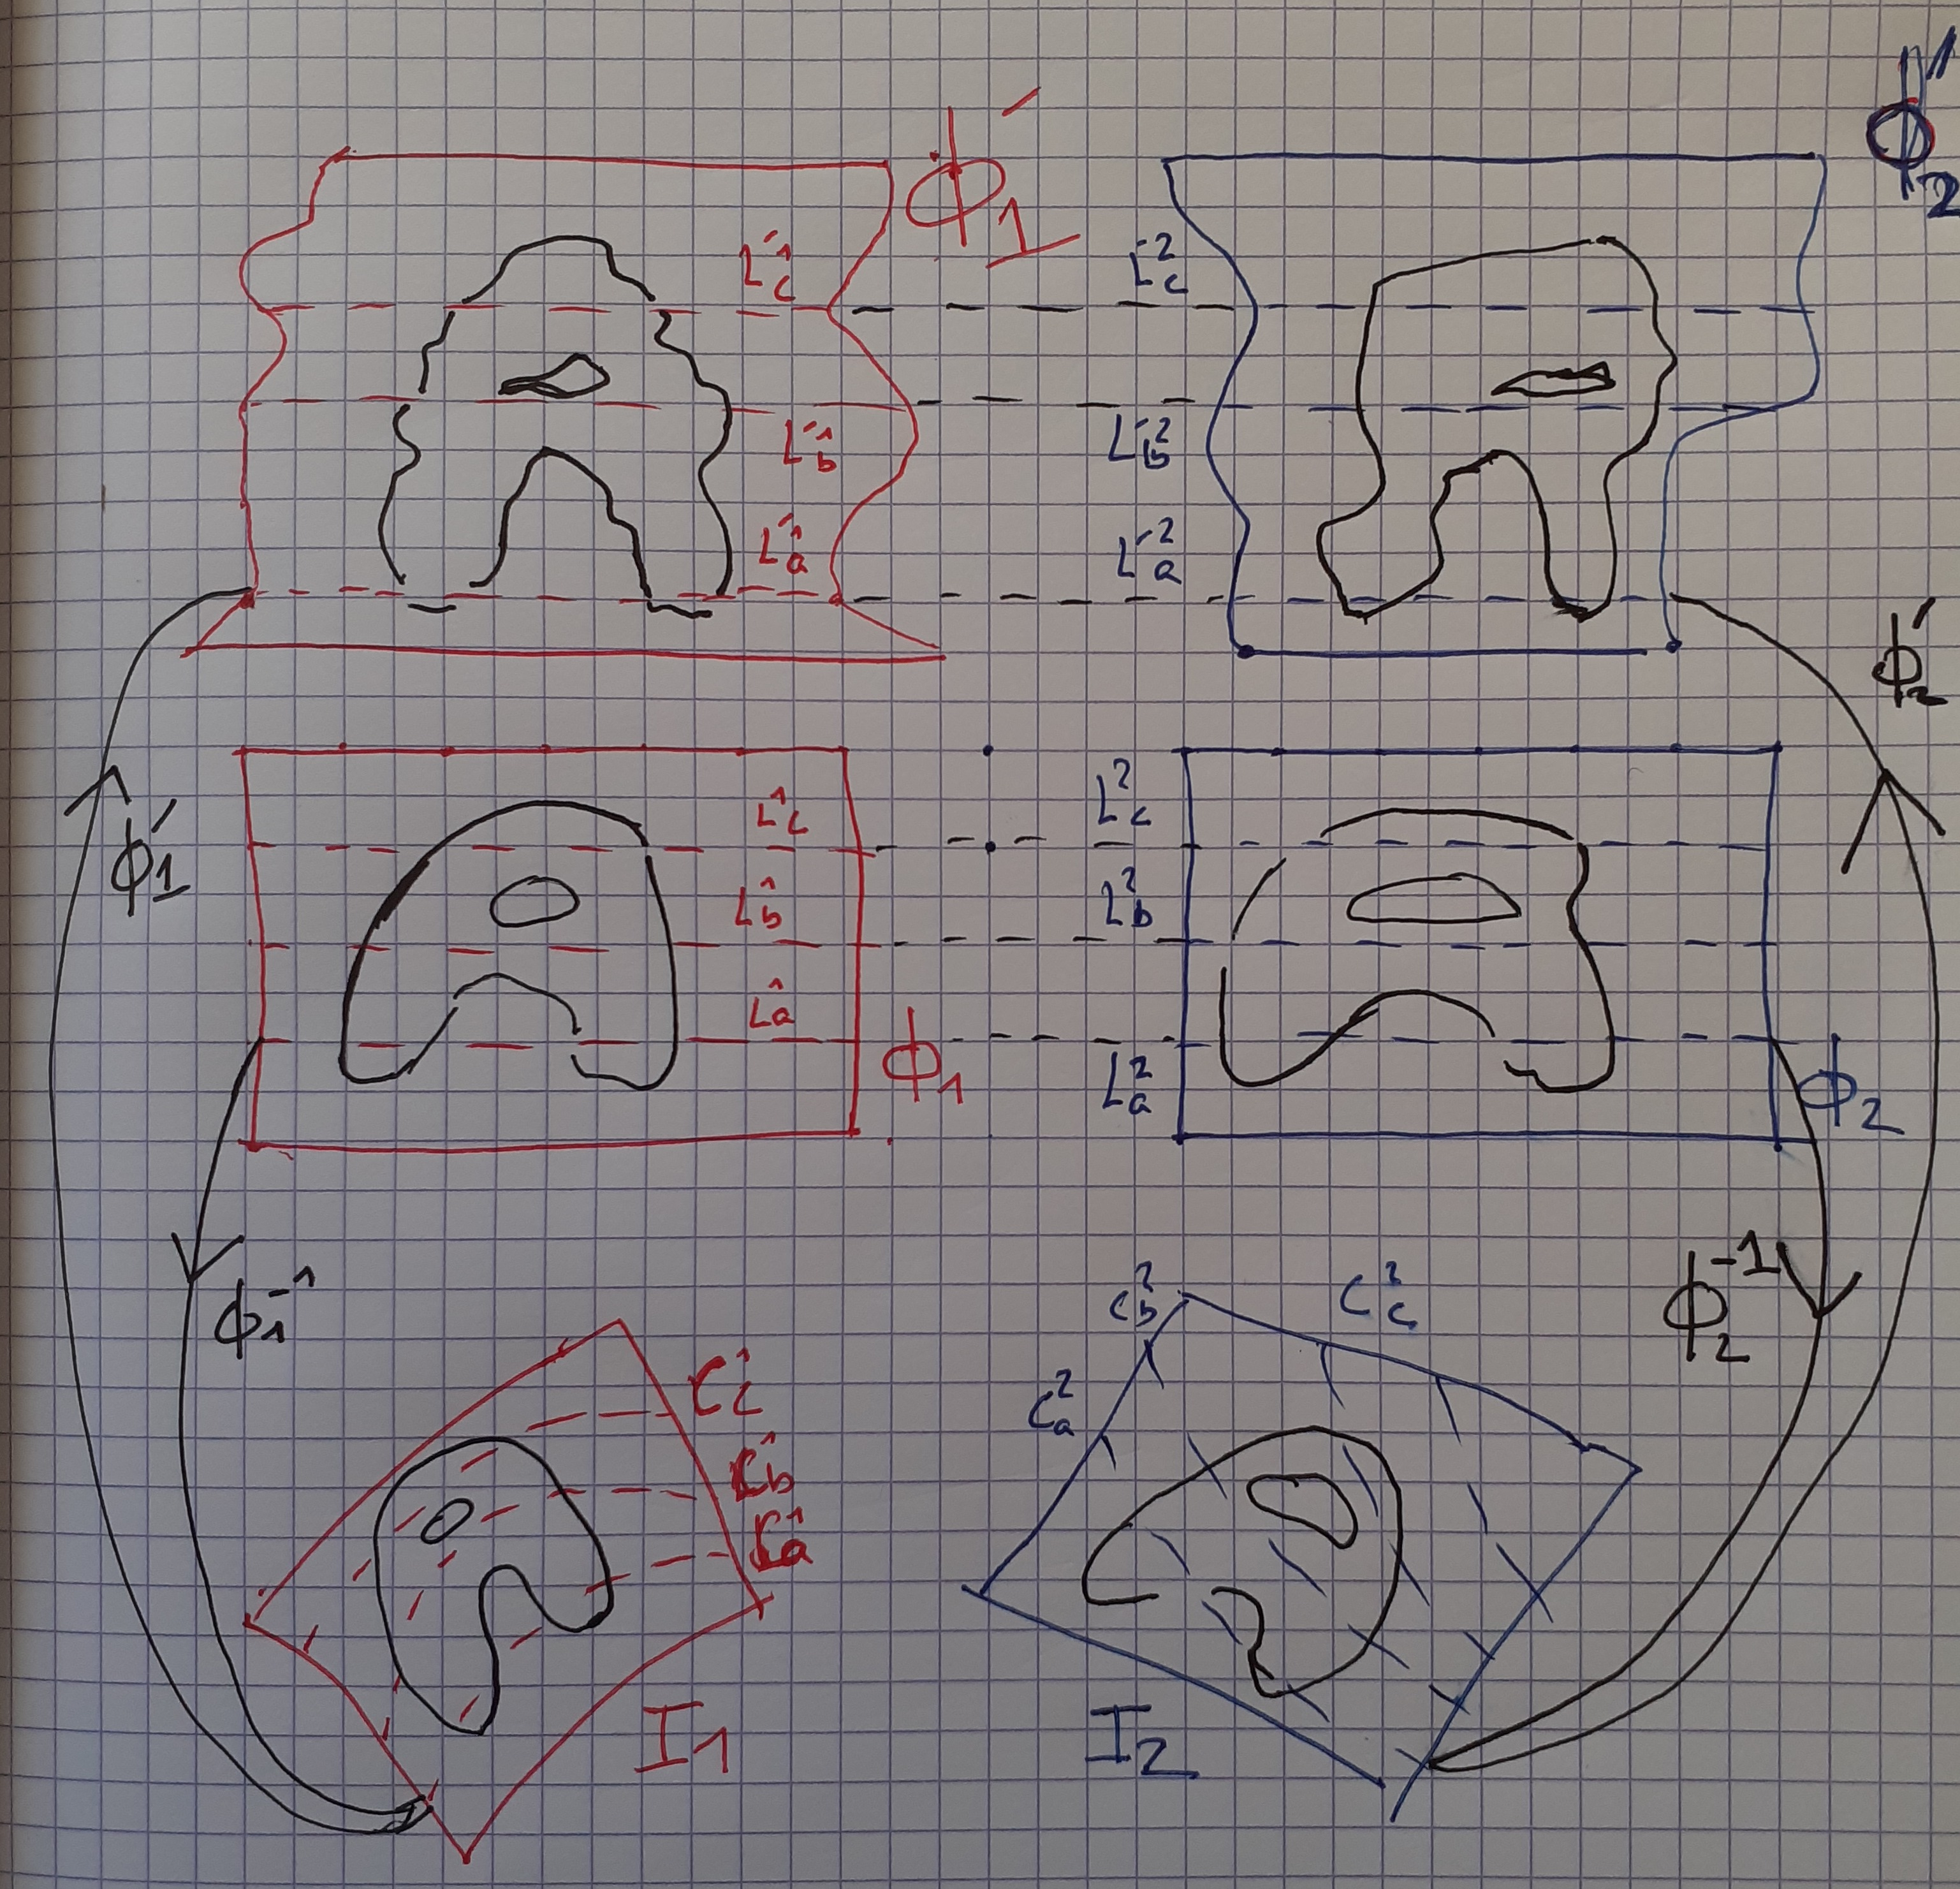
\includegraphics[width=10cm]{FIGS/AmbigEpip.jpg}
 \\ \hline \hline
\end{tabular}
\caption{Ambiguity : two possible epipolar resampling}
\label{FigAmbigEpip}
\end{figure}




\begin{theorem}[Unique epipolar constraint]

If epipolar ressempling exist, there exist a unique epipolar resampling $\phi_1,\phi_2$ satisfying 
the $3$ following constraints:

\begin{equation}
    \phi_1(x,y) = (x,y') \label{Ambig:PhiO}
\end{equation}
\begin{equation}
    \phi_2(x,y) = (x,y') \label{Ambig:PhiT}
\end{equation}
\begin{equation}
    \phi_1(0,y) = (0,y) \label{Ambig:Line}
\end{equation}
\label{Theo:Fix:Ambig}

\end{theorem}



%---------------------------------------------
%---------------------------------------------
%---------------------------------------------

\section{Proposed method for epipolar ressampling}


\subsection{Hypothesis and layout}

\subsubsection{Principles}
The principle of the methods is to use \emph{H-Compatible}  points $p_1,p_2$ to calculate a
pair of function $\phi_1,\phi_2$ that complain with the epipolar constraint :
\emph{"$\phi_1(p_1)$ and $\phi_2(p_2)$ are on the same line"}. As these epipolar function
are not unique, in application of theorem~\ref{Theo:Fix:Ambig} we  parametrize $\phi_k$ according to following equation :


\begin{equation}
    \phi_k(i,j) = (i,V_k(i,j))  \; \; ; \; \;
    V_k : \RR^2 \rightarrow \RR  
  \label{EpipVParam}
\end{equation}

This parametrization handle  equation~\ref{Ambig:PhiO} and~\ref{Ambig:PhiT}; 
we will see later \footnote{see equation~\ref{CstrV1:0} and ~\ref{CstrV1:1} in section~\ref{ChoicePolyn}}
how we handle equation \ref{Ambig:Line}.
For  computing $V_1,V_2$ , for any pair of \emph{H-Compatible} points we add the observation
of equation~\ref{EqV1V2} that constraint $V_1$ and $V_2$ :


\begin{equation}
    V_1(p_1) = V_2(p_2) \label{EqV1V2}
\end{equation}

\subsubsection{Hypothesis}


The method take as input two geometric models of the camera $\pi_1$ and $\pi_2$.
These models are regarded as "black box" satisfying the equation~\ref{Eq:Proj} and the method 
make no specific assumption on the physical model of the camera. In our own \CPP implementation,
the cameras are regarded as pure virtual classes offering interface to equation~\ref{Eq:Proj}.
In this paper, the examples processed by our method are RPC satellite models and frame camera (central perspective) but the
only restriction in on the "smoothness" of the projection function :

\begin{itemize}
    \item the fact that $\pi$ are   $\mathcal{C}^{\infty}$ function;
    \item the fact that the direction of epipolar curves have a limited interval of variation (say for example
          less than $\frac{\pi}{2}$).
\end{itemize}

\begin{figure}
\centering
\begin{tabular}{||c||}
 \hline \hline
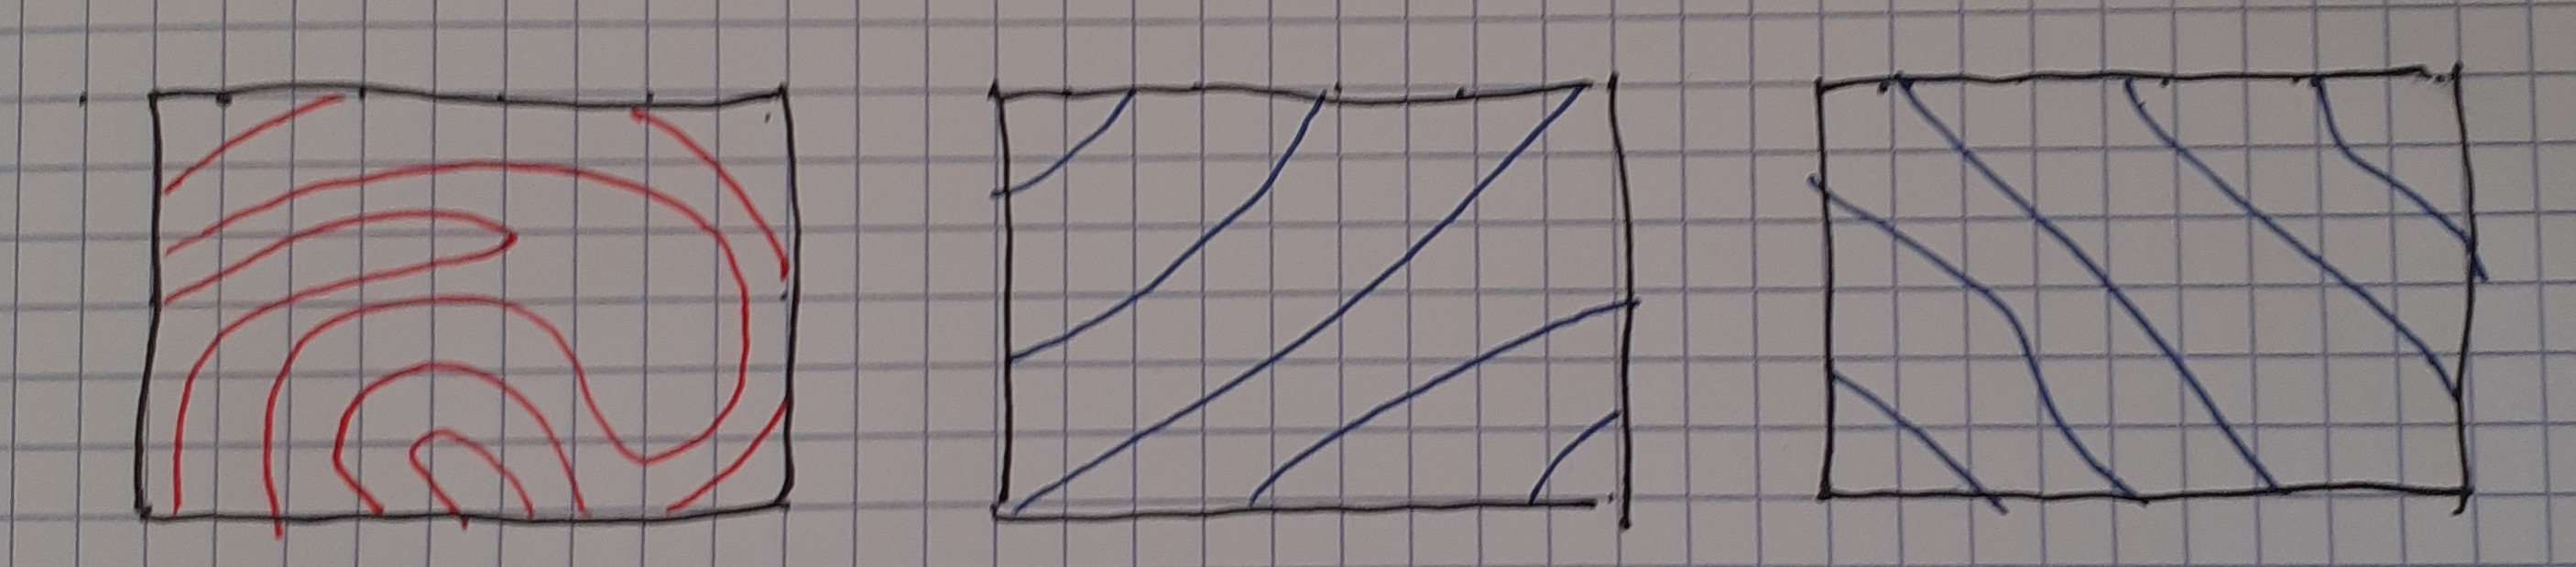
\includegraphics[width=10cm]{FIGS/BadGoodLines.jpg}
 \\ \hline \hline
\end{tabular}
\caption{Left : a set of epipolar line not handled with our methods. Right : a perfectly acceptable pair  of epipolar line}
\label{BadGoodEpip}
\end{figure}

Figure~\ref{BadGoodEpip} illustrates the last constraint on epipolar curves. Left image present a set
of epipolar line that would not be handled by our methods.  Right image, represent a pair of epipolar line
that would be handled without problem because for each of them the direction of the line are included
in a restricted interval. 


\subsubsection{Center and global direction estimations}

The mehod estimate first the center $C_1,C_2$ of set of points $p_1$ and $p_2$, this is done by
a simple computation of average of coordinates.  Then all the computation are done in
a repaire originate in this center. 

This operation is usefull for the  application of constraint~\ref{Ambig:Line} so that is applied
at the center of the data.



The method then estimates for each image the average direction $\vec{D}_k$
of its epolar line, and a rotation $R_k$ is applied to the data so that the epipolar line become
globally horizontal using formula of equation~\ref{EqRot}.
The  epipolar deformation is computed on these rotated data.

\begin{equation}
    R_k(p) =  \frac{p-C_k}{\vec{D}_k}  \label{EqRot}
\end{equation}


This setting in a repair where epipolar lines are globaly horizontal, is
a consequence of equations~\ref{EpipVParam}, and is illustrated by figure~\ref{ReqOrient} :

\begin{itemize}
   \item left image of figure~\ref{ReqOrient} presents a case where epipolar curve are quasi vertical
         and for which an epipolar correction, without initial rotation,  
          according to equation~\ref{EpipVParam} would be impossible;
   \item middle image of figure~\ref{ReqOrient} presents a case where epipolar curve are oblique,
         in this case epipolar correction according to equation~\ref{EpipVParam} would be possible
         but would lead to important distorsion in the image, as can be seen on left image.
\end{itemize}




\begin{figure}
\centering
\begin{tabular}{||c||}
 \hline \hline
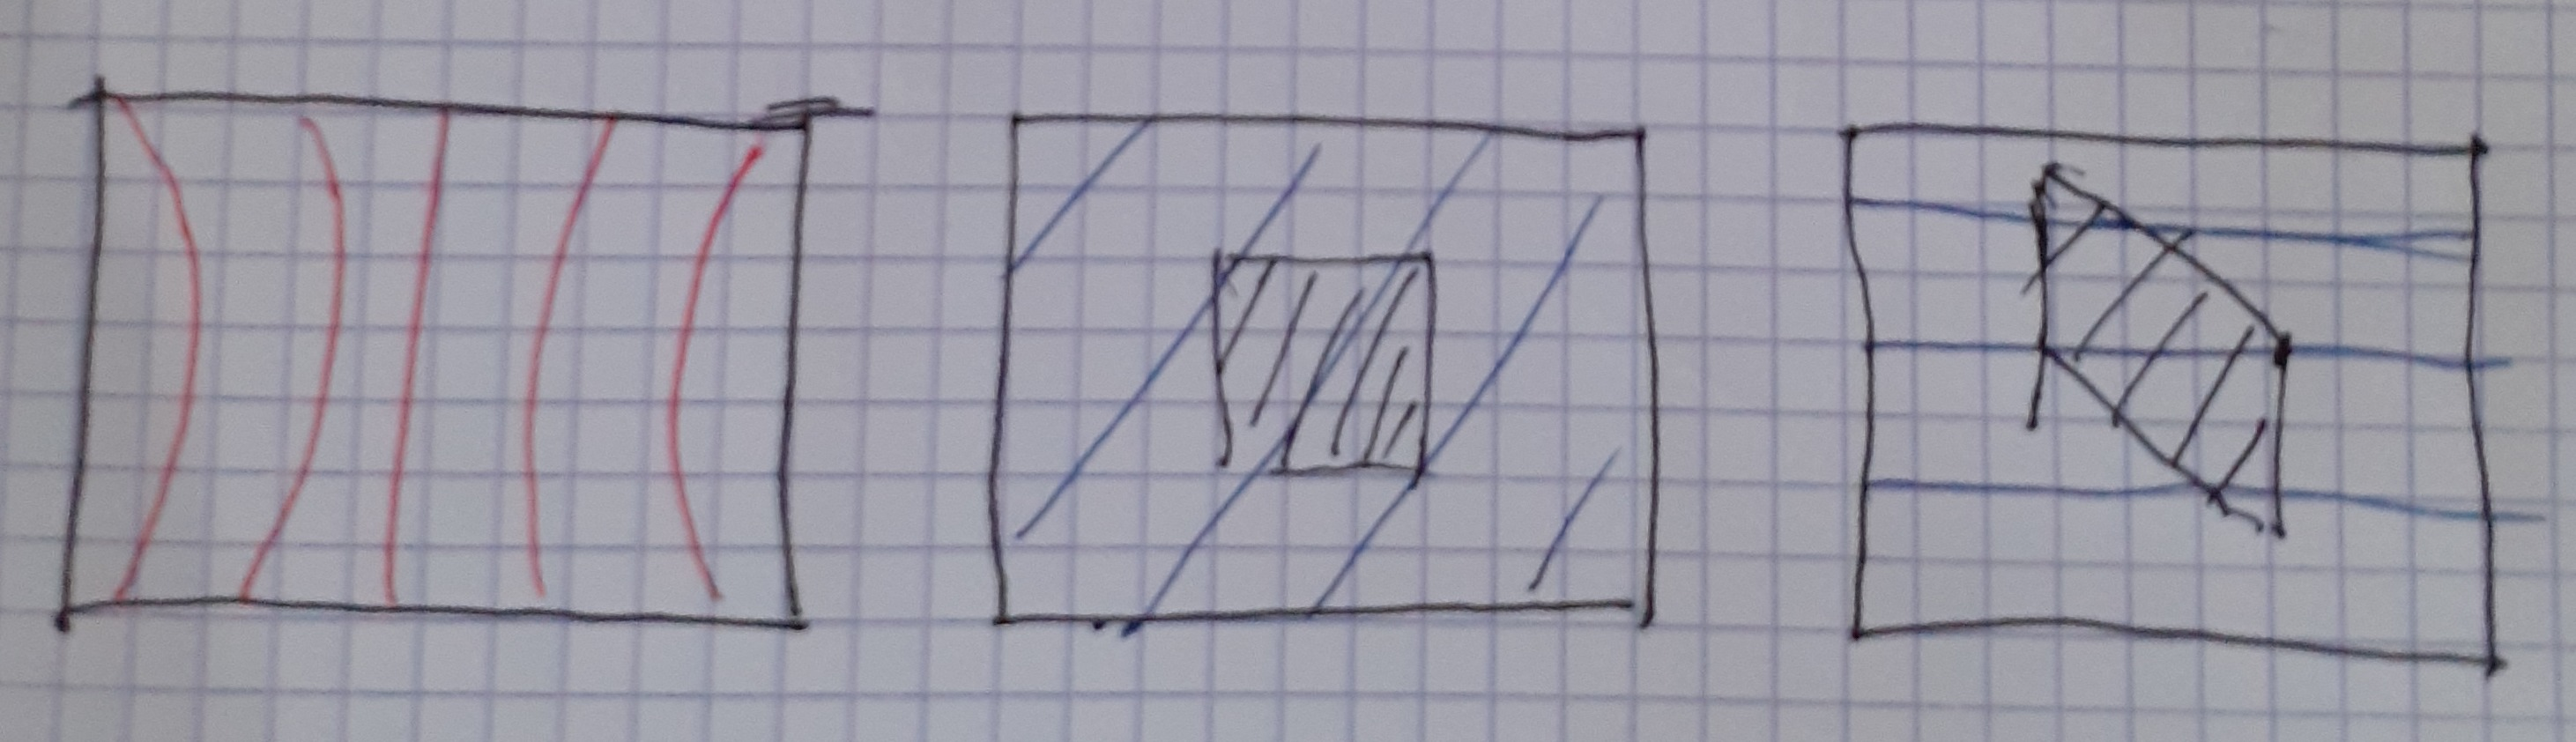
\includegraphics[width=10cm]{FIGS/EpipReqOrient.jpg}
 \\ \hline \hline
\end{tabular}
\caption{Left : quasi vertical epipolar curve, correction with equation~\ref{EpipVParam} is impossible. 
         Middle,Right  : oblique curve, epipolar rectification  with equation~\ref{EpipVParam} is possible
         but generate important distorsion}
\label{ReqOrient}
\end{figure}





\subsubsection{Layout}

The layout of the method we propose is then $3$ steps : (1) estimate the global 
direction of epipolar curve (2) estimate $F_1,F_2$ the local epipolar rectification
 in the repaire linked to these global direction (3)  estimate the final
epipolar rectification as a composition of $F_1,F_2$ and the rotation.
A more formalized description of the algorithm is given in bloc ~\ref{AlgoGlob}.


\begin{algorithm}
\caption{Epipolar($\pi_1$,$\pi_2$)}
\begin{algorithmic}
    \STATE {\emph{Layout of the algorithm for computing the epipolar rectification from camera models}}
    \STATE Use $\pi_1,\pi_2$ to estimate a set of \emph{H-Compatible} point $\mathcal{H} =\{(p_1,p_2)\}$ : 
    \STATE Estimate centers $C_1$ and $C_2$ ;
    \STATE Estimate global direction of epipolars $\vec{D}_1$ and $\vec{D}_2$ ,
    \STATE Estimate rotations $R_1,R_2$ according to formula~\ref{EqRot}
    \FORALL{$p_1,p_2 \in \mathcal{H}$}
              \STATE set : $q_1 = R_1(p_1)$,  $q_2 = R_2(p_2)$
              \STATE add equation : $V_1(q_1) = V_2(q_2)$
    \ENDFOR
    \STATE estimate by least square $V_1$ and $V_2$
    \STATE set $F_k(x,y)=(x,V_k(x,y))$  %, $F_2(x,y)=(x,V_2(x,y))$
    \STATE set $\phi_k =  F_k \circ  R_k $ % and $\phi_2=F_2 \circ R_2$
    \RETURN $(\phi_1,\phi_2)$
\end{algorithmic}
\label{AlgoGlob}
\end{algorithm}



\subsubsection{Why should it work ?}

Intuitively, it may be not obvious that the system of equation~\ref{EqV1V2} is well posed.
In fact, in the case where there would exist a functionnal relation between
$p_1$ and $p_2$ , as $p_1=F(p_2)$,  there would exist infinity of solution
for $(V_1,V_2)$ :   for any function $V: \RR^2 \rightarrow \RR $ we can generate a solution $(V\circ F, V)$ .

\begin{figure}
\centering
\begin{tabular}{||c||}
 \hline \hline
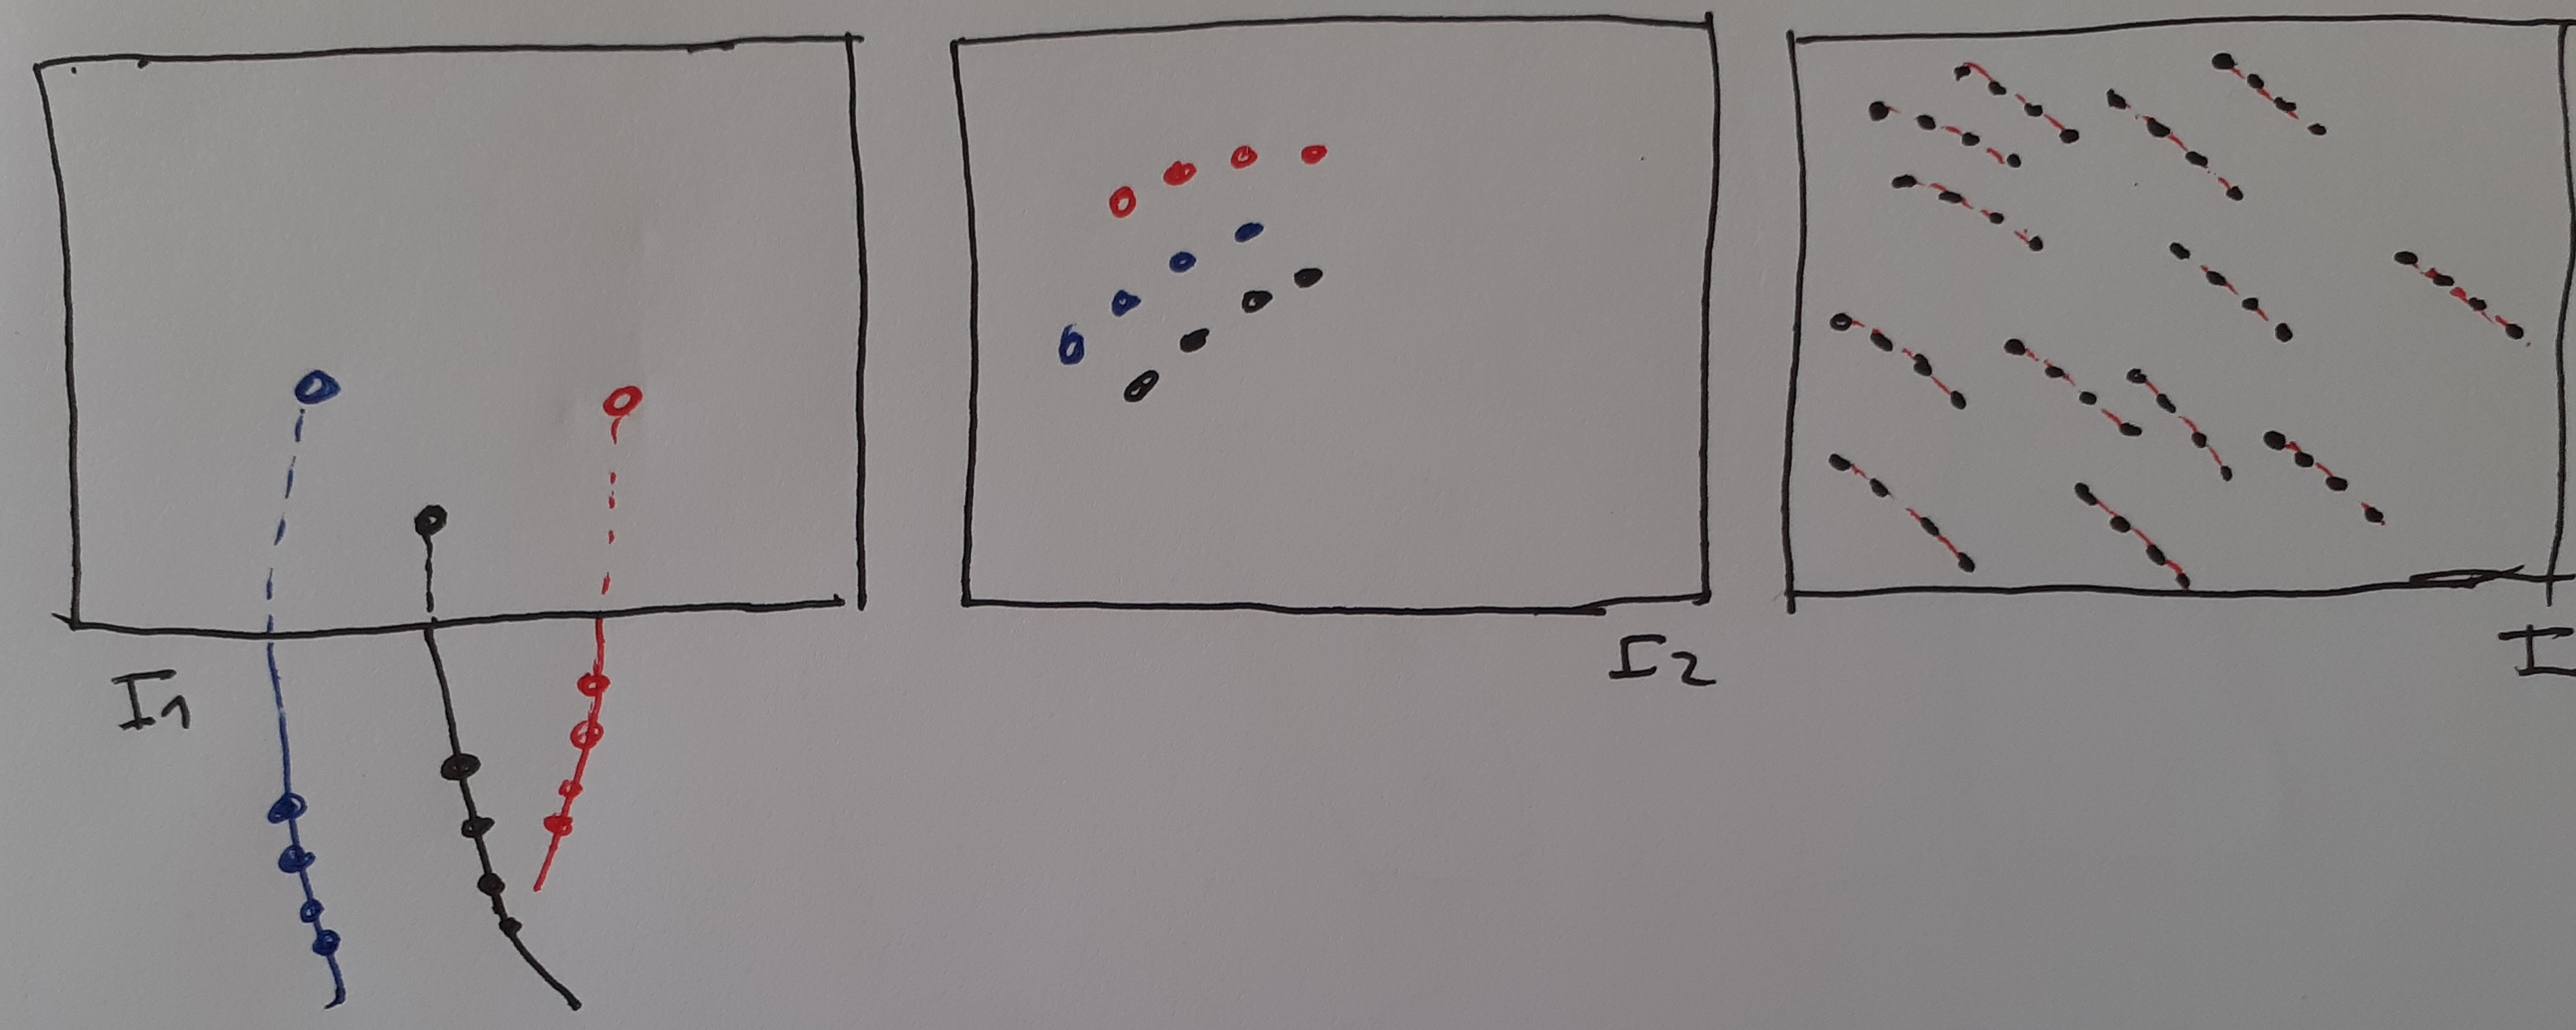
\includegraphics[width=10cm]{FIGS/NonFuncCorresp.jpg}
 \\ \hline \hline
\end{tabular}
\caption{Letft : for each $p_1$ we generate several $3d$ point on $B_1(p_1)$ . Middle :
         the multiple corresspondance in $I_2$ . Right : a dense network of curve in $I_2$.}
 
\label{NonFuncCorresp}
\end{figure}

The thing here is that, due to the $3d$ origin of $p_1,p_2$ there is
\emph{no} functionnal relation between $p_1,p_2$ and there is consequently
much more constraint on $(V_1,V_2)$. Instead of functionnal relation,
we can generate  "one to many" (and  "many to one") correspondance as illustrated on figure~\ref{NonFuncCorresp} .
For example, for a given  point $p_1$, folowing the curve $\pi_2(\BundO(p_1))$ we can generate
several points on the bundle (potentially an infinity) and have then several (many) correspondance
by  $\pi_2$ for a single point. Let write $p^k_2$ be multiple homologous of $p_1$,
we have the equation  :


\begin{equation}
    V_1(p_1) = V_2(p^1_2)   \;;\; V_1(p_1) = V_2(p^2_2)   \;;\; V_1(p_1) = V_2(p^3_2)  \dots \label{MultiTieP}
\end{equation}


And equation~\ref{MultiTieP} brings in fact the constraint : 

\begin{equation}
V_2(p^1_2) = V_2(p^2_2)  =  V_2(p^3_2) \dots \label{RedrCurv}
\end{equation}

If we look at left image of figure~\ref{NonFuncCorresp}, we see that equation~\ref{RedrCurv}
impose the constraints that the "piece of curve" become horizontal.

%---------------------------------------------
%---------------------------------------------
%---------------------------------------------


\subsection{Detailled implementation}


\subsubsection{Choice of a parametric functional space}
\label{ChoicePolyn}

We need to select a space of parametric function to represente $V_1,V_2$. The only constraint
is that $V_1,V_2$ are $\mathcal{C}^{\infty}$ function , plus the additional constraint of 
equation~\ref{Ambig:Line}. 

Classicaly when we want to parametrize a set of function  $\mathcal{C}^{\infty}$,
a "natural" candidate is the set of polynoms of given degree; we know the function will be
$\mathcal{C}^{\infty}$ and, according to Stone-Weierstrass theorem (\cite{Weierstrass1885} and \cite{Stone1937})
which says that they space of polynoms is dense in the space of continuous function, we know that a suffucient
degree we will be abble to approximate any function with the desirable accuracy. A possible
limitation of selecting polynomal with high degree is over-fitting that may lead to
undesirable high frequency; we dont have this problem here because  the measure
are synthetized from $\pi_1,\pi_2$ and, whatever beign the degree we select for polynomial,
we can add sufficient number of measure to have a high level of redundancy (say, for example
$100$ times more measures than constraints).

Let $d$ be the selected degree, we have two vectors of unknown $C^1_{a,b},C^2_{a,b}$ 
corresponding to coefficients of the polynoms as written in equation~\ref{EqPol}:


\begin{equation}
   V_k(p) = V_k(i,j) =  \sum\limits_{\substack{a=0}}^d  \sum\limits_{\substack{b=0}}^{d-a}  C^k_{a,b}  i^a j^b \label{EqPol}
\end{equation}
   
\subsubsection{Imposing constrainte on global lines deformation}

In this paramatrisation, we must take into account equation~\ref{Ambig:Line}.
When using constraint~\ref{Ambig:Line}, we have  $i=0$ , so we can supress all term  $i^a$ for $a\neq 0$
and the equation can be writen as :


\begin{equation}
    V_1(0,j) =  j =   \sum\limits_{\substack{b=0}}^{N}  C^1_{0,b}  j^b  \label{CstrV1:0}
\end{equation}

In equation~\ref{CstrV1:0}, $j$ and the  sum are both polynom, so if their function are equal on a segment, they
must be equal term by term. The constraint then comes to force a number the
unknown $C^1_{0,k}$ who have a known value  : $1$ for $C^1_{0,1}$ and $0$ else.
Using kronecker delta we can write :

\begin{equation}
         C^1_{0,k} = \delta_{1,k} \label{CstrV1:1}
\end{equation}

\subsubsection{Generation of points, direction and centers}

The generation of  data from $\pi_1$ and $\pi_2$  is made
in two way, once with $I_1$ as master, once with $I_2$;
at each step the  "master one" is 
used to follow its bundle. The algorithm~\ref{AlgoGenData} present the 
generation of the points with $\pi_1$  as master.

\begin{algorithm}
\emph{Compute a list $L_{1,2}$  of   $\pi_1-\pi_2$ H-compatible pair with $I_1$ as master image,
  compute also center $c_1$ of points of $I_1$  and global direction $\vec{D}_2$ for epipolar curves of $I_2$}
\caption{GenerateData()}
\begin{algorithmic}
    \STATE $L_{1,2}\gets () $ ;  $c_1 \gets (0,0)$  ;   $\vec{D}_2 \gets  \overrightarrow{(0,0)}$ ; $N \gets 0 $
    \FOR{$p_1.x=0$  \TO $X_1$  {\bf Step} $\delta_{x,y}$   } 
        \FOR{$p_1.y=0$  \TO $Y_1$  {\bf Step} $\delta_{x,y}$    } 
             \FOR{$z=Z_0$  \TO $Z_1$  {\bf Step} $\delta_{z}$   } 
                  \STATE {$p_2 = \pi_2(\PiVert^{-1}_1(p_1,Z))$}
                  \STATE {$p'_2 = \pi_2(\PiVert^{-1}_1(p_1,Z+\delta_{z}))$}
                  \IF {$p_2 \in I_2$ \AND $p'_2 \in I_2$}
                       \STATE $L_{1,2}.append((p_1,p_2))$  
                       \STATE $c_1 \gets c_1 + p_1$
                       \STATE $\vec{D}_2 \gets  \vec{D}_2 + \frac{\overrightarrow{p_2 p'_2}}{|p_2 p'_2|}$
                       \STATE $N \gets  N +1 $
                  \ENDIF
             \ENDFOR
        \ENDFOR
    \ENDFOR
    $c_1 \gets \frac{c_1}{N}$  ; $\vec{D}_2 \gets \frac{\vec{D}_2}{N} $
\end{algorithmic}
\label{AlgoGenData}
\end{algorithm}

\ref{PiInvert}


\subsubsection{Using center and direction}

Once we have computed centers $c_1,c_2$, directions   $\vec{D}_1,\vec{D}_2$  and the list $L_{1,2}$,
we use it  to normalize the center the measure and make the direction globally
horizontal : we apply equation~\ref{EqRot}  to all elements of the list.


\subsubsection{Estimating the rectification}

As the data are synthetic data, without outlayer, we can directly solve
the equations by least square . This essentially is
a matter of merging the previous part :

\begin{itemize}
    \item let $d$ be the degree of the polynoms;
    \item the unknown are the coefficient of the polynomes $V_1$ and $V_2$, there is
          $\frac{(d+1)(d+2)}{2}$ unknowns for $V_2$ and $\frac{(d+1)(d+2)}{2}-(d+1) $  for $V_1$
          taking into account the  constraint of equation ~\ref{CstrV1:1}
     \item for each pair of corrected point $q_1,q_2$ we add to the least square system
          the equation ~\ref{EqPol};
\end{itemize}

We then estimate the $V_1,V_2$ by in the least square system. An obtain :

\begin{equation}
  \varphi_k(p) = \varphi_k(i,j) = (i,V_k(i,j))  \;;\;    \phi_k =  \varphi_k  \circ R_k 
\end{equation}

\subsubsection{Estimating inverse function}

For the computation of the rectified image itself, we also need the inverse function, 
as the natural way to resample  $I_k$ in $E_k$ is to write :

\begin{equation}
  E_k(p) = I_k(\phi^{-1}_k(p))
\end{equation}

The inverse of $R_k$ is obvious. For computing the inverse of $\varphi_k$  we
use the fact that if $\varphi$ is invariant for the column, then $\varphi^{-1}$ is also.
So we can paremetrize it with a function $W : \RR^2 \rightarrow \RR$ as :

\begin{equation}
  \varphi^{-1}_k(p) = \varphi^{-1}_k(u,v) = (u,W_k(u,v))  
\end{equation}


For the estimation of $W$ we use the same argument as in~\ref{ChoicePolyn}, and
use the base of polynomial function. Once the $V_k$ are known we generate
for each point $p_k=(i,j)$ in $L_{1,2}$ the observation :

\begin{equation}
   W_k(i,V_k(i,j))  = j \label{InverseEpip}
\end{equation}

If we want to assure that the computed inverse is sufficiently close
to the "real" inverse we can increase the degre (typically the degree of $W$
is $d+4$ in our implementation). These has no inconvenient as long the redunduncy
is high enough.


%---------------------------------------------
%---------------------------------------------
%---------------------------------------------

\section{Experimentation}

Exemple de résultats avec résidus. + qq crop d'images rectifiees.

\subsection{Use with satellite images}

C'est la que c'est vraiment utile .... 


\subsection{Use with pinhole camera}

Permet de faire des test supplémentaire.

\subsection{Use without model}


Exposé precis avec modele analytique:

    * calcul des points homologues, en 3D => direction moyenne
    * resolution par moindres carress avec degres élevé, degré sup pour l'inverse
    * Utilité du 3D, precision en fonction de la nappes, possibilité d'utiliser un modèle 3D grossier .

In its standard use
    
%---------------------------------------------
%---------------------------------------------
%---------------------------------------------

\section{Discussion and perspective}

Avantage de la methode : modeles analyique, minimise deformation et residu, peut être appliquee 
si on a que les points homologues (photo escalier ?).

Inconvenient ? Cas comme \ref{BadGoodEpip} pas gere, peut être le sont il par Oh ?

Future work => use MNT ? Test sur configuration plus compliquées : orbites differentes ? Radar ? Radar/visible ?






%---------------------------------------------
%---------------------------------------------
%---------------------------------------------



\begin{thebibliography}{References}
   \bibitem[Oh,     Jaehong. 2011]{Oh2011}
            Oh,     Jaehong. 2011,     Novel     Approach     to     Epipolar Resampling  of  
            HRSI  and  Satellite  Stereo  Imagery-based Georeferencing   of   Aerial   Images.Diss.
            The   Ohio   State University.

   \bibitem[De Franchis,Carlo 2015]{Franchis2015}   Earth Observation and Stereo Vision.
           Ph Dissertation, Paris-Saclay 2015.

    \bibitem[Weierstrass,Karl 1885 ]{Weierstrass1885} Über die analytische Darstellbarkeit sogenannter willkürlicher Functionen 
           einer reellen Veränderlichen. Sitzungsberichte der Königlich Preußischen Akademie der Wissenschaften zu Berlin, 
           1885 (II).  Erste Mitteilung (part 1) pp. 633–639, Zweite Mitteilung (part 2) pp. 789–805.

    \bibitem[Stone, M. H. 1937]{Stone1937} "Applications of the Theory of Boolean Rings to General Topology", 
          Transactions of the American Mathematical Society, Transactions of the American Mathematical Society, 
          Vol. 41, No. 3, 41 (3): 375–481
\end{thebibliography}

\end{document}






